\chapter{Experiments}
\label{chap:experiments}
% ここから、ここから

\section{Two-dimensional Rotating-Hill Heat Equation}
\label{sec:moving-hill-dwr}

This section shows the complete DWR adaptive workflow for a time-dependent two-dimensional heat equation. The example is a manufactured benchmark with a localised temperature peak that moves around the domain. It is therefore well suited to testing whether a space--time error indicator identifies both the spatial location of the peak and the time intervals in which an accurate representation is required.

We compare with two goal-oriented adaptive strategies: one based on a manually derived residual localisation and one based on the automated bubble--cone recovery developed in Section~\ref{sec:space-time-residual-recovery}.


\subsection{Manufactured Problem and Quantity of Interest}
Let $\Omega=(0,1)^2$, let $T=1$, and write $Q:=\Omega\times(0,T)$. We consider the heat equation
\begin{equation}
  \partial_t u-\Delta u=f
  \quad\text{in }Q,
  \qquad
  u=u_{\mathrm{ex}}
  \quad\text{on }\partial\Omega\times(0,T],
  \qquad
  u(\cdot,0)=u_{\mathrm{ex}}(\cdot,0).
  \label{eq:mh-primal}
\end{equation}
The source term $f$ is chosen by the method of manufactured solutions so that the exact solution is
\begin{equation}
  u_{\mathrm{ex}}(x,y,t)
  =
  \frac{1}{1+\alpha r^2(x,y,t)},
  \qquad
  r^2(x,y,t)
  =
  (x-c_x(t))^2+(y-c_y(t))^2,
  \label{eq:mh-exact}
\end{equation}
where $\alpha=50$ and
\begin{equation}
  (c_x(t),c_y(t))
  =
  \left(
    \frac12+\frac14\cos(2\pi t),
    \frac12+\frac14\sin(2\pi t)
  \right).
  \label{eq:mh-centre}
\end{equation}
Thus $u_{\mathrm{ex}}$ is a smooth, localised hill whose centre travels once around a circle of radius $1/4$ about the centre of the unit square. Although the solution remains smooth, its strongest spatial variation is concentrated near the moving peak.

The reference rotating-hill benchmark uses the space--time $L^2$ error to measure how well the local behaviour of the solution is captured \cite{ThieleWick2024}. Here we use its squared, differentiable counterpart. More precisely, we define the manufactured-error or space--time tracking functional
\begin{equation}
  J(v)
  :=
  \frac12\int_0^T\!\int_\Omega
  \bigl(v-u_{\mathrm{ex}}\bigr)^2
  \,\mathrm{d}x\,\mathrm{d}t.
  \label{eq:mh-goal}
\end{equation}
For the numerical solution $u_h$,
\begin{equation}
  J(u_h)
  =
  \frac12
  \lVert u_h-u_{\mathrm{ex}}\rVert_{L^2(Q)}^2.
  \label{eq:mh-goal-error}
\end{equation}
This quantity measures the cumulative mean-square discrepancy between the computed and exact temperature fields over the whole space--time cylinder. It penalises errors in the position, height, and shape of the moving peak, as well as errors accumulated during its motion. It is therefore an appropriate diagnostic goal for assessing space--time mesh adaptation in a manufactured-solution experiment.

Since
\begin{equation}
  J'(u_h)(v)
  =
  \int_0^T\!\int_\Omega
  (u_h-u_{\mathrm{ex}})v
  \,\mathrm{d}x\,\mathrm{d}t.
  \label{eq:mh-goal-derivative}
\end{equation}
Accordingly, the continuous adjoint used for verification is
\begin{equation}
  -\partial_t z-\Delta z
  =
  u_h-u_{\mathrm{ex}}
  \quad\text{in }Q,
  \qquad
  z=0
  \quad\text{on }\partial\Omega\times(0,T),
  \qquad
  z(\cdot,T)=0.
  \label{eq:mh-adjoint}
\end{equation}
The homogeneous adjoint boundary condition follows because variations of the primal solution vanish on the strongly imposed inhomogeneous Dirichlet boundary. The terminal condition arises from integration by parts in time: the primal problem is an initial-value problem, whereas its adjoint is solved backwards from $T$.

% For our numerical experiment, the primal approximation uses $\mathrm{CG}(1)\times\mathrm{DG}(0)$. The low-order dual is computed in the same space, while the enriched dual uses $\mathrm{CG}(2)\times\mathrm{DG}(1)$. The computable DWR weight is
% \begin{equation}
%   z^\star
%   =
%   z_{\mathrm{enriched}}-z_{\mathrm{low}}.
%   \label{eq:mh-dwr-weight}
% \end{equation}


\subsection{Two Refinement Indicators}

% \paragraph{Uniform baseline.}
% The uniform run provides a non-adaptive reference sequence. At each iteration, every spatial cell on every time slab is refined and every time slab is bisected. For the triangular meshes used here, one spatial cell therefore produces four children, while bisection of the time partition produces two child slabs. Consequently, the number of space--time cells increases by approximately a factor of eight at each uniform refinement step.

\paragraph{Strong-residual marking score.\cite{Bangerth_Rannacher_2003,Becker_Rannacher_2001}}
For comparison, we construct a positive residual-based activity using the classical strong residual representation for the heat equation. On a space--time cell $Q_{K,n}=K\times I_n$, define
\begin{equation}
  R_{K,n}
  :=
  f+\nabla\cdot(\kappa\nabla u_h)-\partial_tu_h,
  \label{eq:mh-strong-cell-residual}
\end{equation}
and, on an interior spatial facet $F\subset\partial K$,
\begin{equation}
  r_{K,F,n}
  :=
  \frac12\llbracket\kappa\nabla u_h\cdot n\rrbracket.
  \label{eq:mh-strong-facet-residual}
\end{equation}
The factor assigns half of the flux jump to each adjacent cell. For the strongly imposed Dirichlet condition in \cref{eq:mh-primal}, no additional boundary-facet residual is present.

The starting point is the local strong residual action
\begin{align}
  \rho_{K,n}(v)
  ={}&
  (R_{K,n},v)_{K\times I_n}
  -\sum_{F\subset\partial K}
   (r_{K,F,n},v)_{F\times I_n} -
  \bigl([u_h]_{n-1},v(t_{n-1}^{+})\bigr)_K,
  \label{eq:mh-strong-residual-action}
\end{align}
where the last term is the dG time-interface contribution. Pairing this action with the dual error and applying the Cauchy--Schwarz inequality separately to the volume, spatial-facet, and temporal-interface terms gives
\begin{subequations}
\begin{align}
  \bigl|(R_{K,n},z^\star)_{K\times I_n}\bigr|
  &\leq
  \lVert R_{K,n}\rVert_{K\times I_n}
  \lVert z^\star\rVert_{K\times I_n},
  \label{eq:mh-volume-cauchy}
  \\
  \bigl|(r_{K,F,n},z^\star)_{F\times I_n}\bigr|
  &\leq
  \lVert r_{K,F,n}\rVert_{F\times I_n}
  \lVert z^\star\rVert_{F\times I_n},
  \label{eq:mh-facet-cauchy}
  \\
  \bigl|([u_h]_{n-1},z^\star(t_{n-1}^{+}))_K\bigr|
  &\leq
  \lVert [u_h]_{n-1}\rVert_K
  \lVert z^\star(t_{n-1}^{+})\rVert_K.
  \label{eq:mh-time-cauchy}
\end{align}
\end{subequations}
To combine volume and facet quantities with compatible scaling, we insert the factors $h_K^{-1/2}h_K^{1/2}=1$. Likewise, $k_n^{-1/2}k_n^{1/2}=1$ gives the natural scaling for the temporal jump. This yields
\begin{subequations}
\begin{align}
  \rho_{K,n}^{1}
  &:=
  \lVert R_{K,n}\rVert_{K\times I_n}
  +
  h_K^{-1/2}
  \lVert r_{K,F,n}\rVert_{\partial K\times I_n},
  \label{eq:mh-strong-rho-one}
  \\
  \zeta_{K,n}^{1}
  &:=
  \lVert z^\star\rVert_{K\times I_n}
  +
  h_K^{1/2}
  \lVert z^\star\rVert_{\partial K\times I_n},
  \label{eq:mh-strong-zeta-one}
  \\
  \rho_{K,n}^{2}
  &:=
  k_n^{-1/2}\lVert [u_h]_{n-1}\rVert_K,
  \\
  \zeta_{K,n}^{2}
  &:=
  k_n^{1/2}
  \lVert z^\star(t_{n-1}^{+})\rVert_K.
  \label{eq:mh-strong-rho-zeta-two}
\end{align}
\end{subequations}
The resulting non-negative marking activity is
\begin{equation}
  m_{K,n}^{\mathrm{str}}
  :=
  \rho_{K,n}^{1}\zeta_{K,n}^{1}
  +
  \rho_{K,n}^{2}\zeta_{K,n}^{2}.
  \label{eq:mh-strong-score}
\end{equation}

\paragraph{Bubble--recovery localisation.}
The automated method instead reconstructs the weak residual directly from its action on local bubble and cone test functions. For the present $\mathrm{CG}(1)\times\mathrm{DG}(0)$ heat discretisation, the recovered residual has three relevant supporting entities: a volume contribution on $K\times I_n$, a spatial-facet contribution on $F\times I_n$, and a left temporal-face contribution on $K\times\{t_{n-1}\}$. Their cell--slab contribution is
\begin{equation}
  \eta_{K,n}
  =
  \eta_{\mathrm{vol},K,n}
  +
  \eta_{\mathrm{space},K,n}
  +
  \eta_{\mathrm{time},K,n}.
  \label{eq:mh-bubble-signed}
\end{equation}
The quantity used for marking is
\begin{equation}
  m_{K,n}^{\mathrm{bubble}}
  :=
  |\eta_{K,n}|.
  \label{eq:mh-bubble-marker}
\end{equation}


\subsection{Results and Interpretation}

The manufactured moving-hill problem was solved on $\Omega=(0,1)^2$ over $[0,1]$, with initial mesh parameter $n_x=n_y=8$, $N_t=8$ initial time slabs, and $\mathrm{CG}(1)\mathrm{dG}(0)$ primal and $\mathrm{CG}(2)\mathrm{dG}(1)$ enriched spaces. All estimators used the same quadrature rule (seven time quadrature points) and the nonlinear DWR identity for the quadratic running goal~\eqref{eq:mh-goal-error}. Thus, though the heat equation is linear, the estimator accounts for the nonlinearity of the goal functional. The strong-residual bound and the bubble localisation both used global bulk marking with $\theta=0.4$, the within-slab trigger $10\%$, and independent slabwise mesh refinement. Both adaptive sequences have nine reported levels. 
\begin{table}[h]
  \centering
  \begin{tabular}{llrrrrrr}
    \toprule
    method & it. & $N_{\rm st}$ & $N_{\rm cell}$ & $N_t$
           & $J(u_{\rm ex})-J(u_h)$ & $\eta_{\rm global}$ & $I_{\rm eff}$\\
    \midrule
    strong & 0 & 688     & 1,104   & 8  & $-1.638\mathrm{e}{-3}$ & $-1.517\mathrm{e}{-3}$ & 0.9262\\
    strong & 2 & 1,036   & 1,800   & 8  & $-1.512\mathrm{e}{-3}$ & $-1.397\mathrm{e}{-3}$ & 0.9241\\
    strong & 4 & 7,444   & 14,204  & 20 & $-3.579\mathrm{e}{-4}$ & $-3.504\mathrm{e}{-4}$ & 0.9789\\
    strong & 6 & 45,923  & 90,258  & 43 & $-8.678\mathrm{e}{-5}$ & $-8.627\mathrm{e}{-5}$ & 0.9941\\
    strong & 8 & 295,517 & 587,271 & 90 & $-2.079\mathrm{e}{-5}$ & $-2.075\mathrm{e}{-5}$ & 0.9982\\
    \midrule
    bubble & 0 & 688     & 1,104   & 8  & $-1.638\mathrm{e}{-3}$ & $-1.517\mathrm{e}{-3}$ & 0.9262\\
    bubble & 2 & 1,281   & 2,290   & 8  & $-1.492\mathrm{e}{-3}$ & $-1.378\mathrm{e}{-3}$ & 0.9236\\
    bubble & 4 & 9,008   & 17,366  & 18 & $-3.852\mathrm{e}{-4}$ & $-3.766\mathrm{e}{-4}$ & 0.9776\\
    bubble & 6 & 59,663  & 117,833 & 36 & $-1.005\mathrm{e}{-4}$ & $-9.980\mathrm{e}{-5}$ & 0.9934\\
    bubble & 8 & 401,953 & 800,335 & 72 & $-2.541\mathrm{e}{-5}$ & $-2.536\mathrm{e}{-5}$ & 0.9980\\
    \bottomrule
  \end{tabular}%
  \caption{Selected adaptive iterations for the strong-residual bound and bubble localisation. Here $N_{\rm st}=\sum_{n=1}^{N_t}\dim(\mathrm{CG}(1;\mathcal T_n))$, $N_{\rm cell}=\sum_{n=1}^{N_t}\#\mathcal T_n$.}
  \label{tab:moving-hill-selected-iterations}
\end{table}

% trend, I_eff, DoF
Table~\ref{tab:moving-hill-selected-iterations} shows two distinct phases. From iteration $0$ to iteration $2$, both methods retain $N_t=8$ time slabs. The refinement is predominantly spatial. After temporal marking becomes active, the error decreases much more rapidly. For the strong-residual run, $N_t$ grows from $8$ at iteration $2$ to $43$ at iteration $6$, at which point the goal error is below $10^{-4}$. The bubble run increases from $8$ to $36$ slabs over the same iterations and reaches $1.005\times10^{-4}$. At the final reported iteration, the strong and bubble methods attain goal errors of $2.079\times10^{-5}$ and $2.541\times10^{-5}$, respectively.

Both effectivity indices are initially approximately $0.926$, and approach one monotonically after time refinement becomes active. The convergence of $I_{\rm eff}$ to one confirms that the DWR identity correctly estimates the quadratic goal error.

At iteration $8$, the strong-residual run uses 90 time slabs and $2.96\times10^5$ slabwise primal DoFs, whereas the bubble run uses 72 time slabs and $4.02\times10^5$ slabwise primal DoFs. Thus, for the present parameters, the strong-residual strategy attains a slightly smaller goal error with fewer slabwise unknowns. These counts also indicate a different allocation of the refinement budget. The strong-residual method performs more temporal refinement, but retains fewer spatial unknowns per slab on average, suggesting that its spatial refinement is concentrated in smaller regions. This interpretation is consistent with the mesh snapshots below, in which the strong-residual meshes exhibit compact refined patches around the moving hill, whereas the bubble meshes show a more spatially distributed refinement pattern.

\begin{figure}[h]
  \centering
  \begin{subfigure}[b]{0.245\textwidth}
    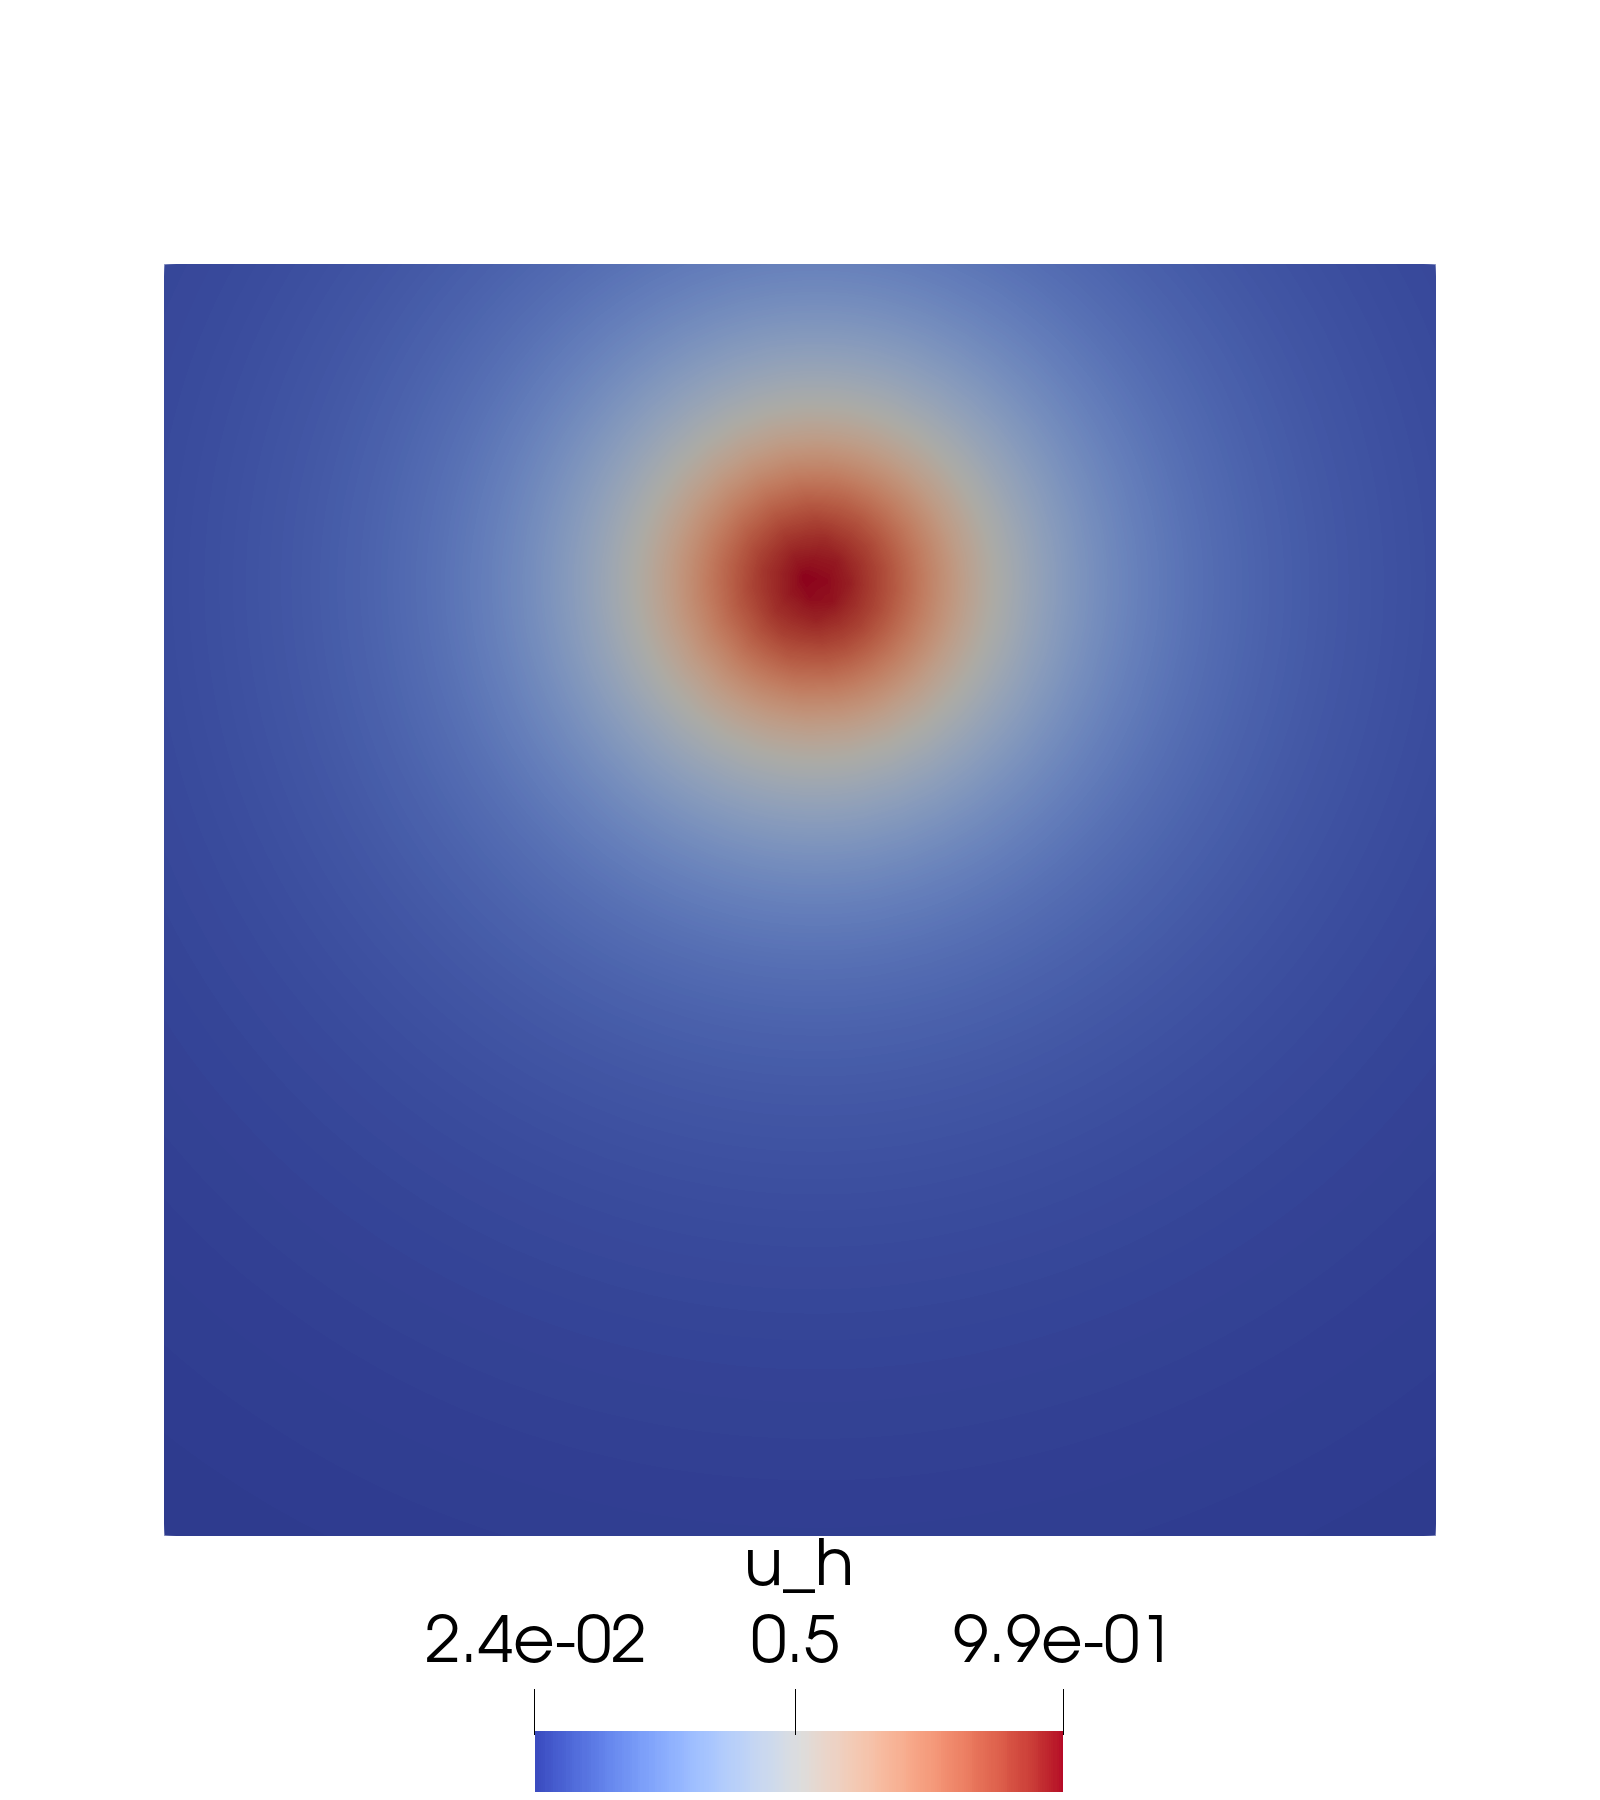
\includegraphics[width=\linewidth]{figures/heat/heat_sol.0000.png}
    \caption{$t=0.25$}
  \end{subfigure}\hfill
  \begin{subfigure}[b]{0.245\textwidth}
    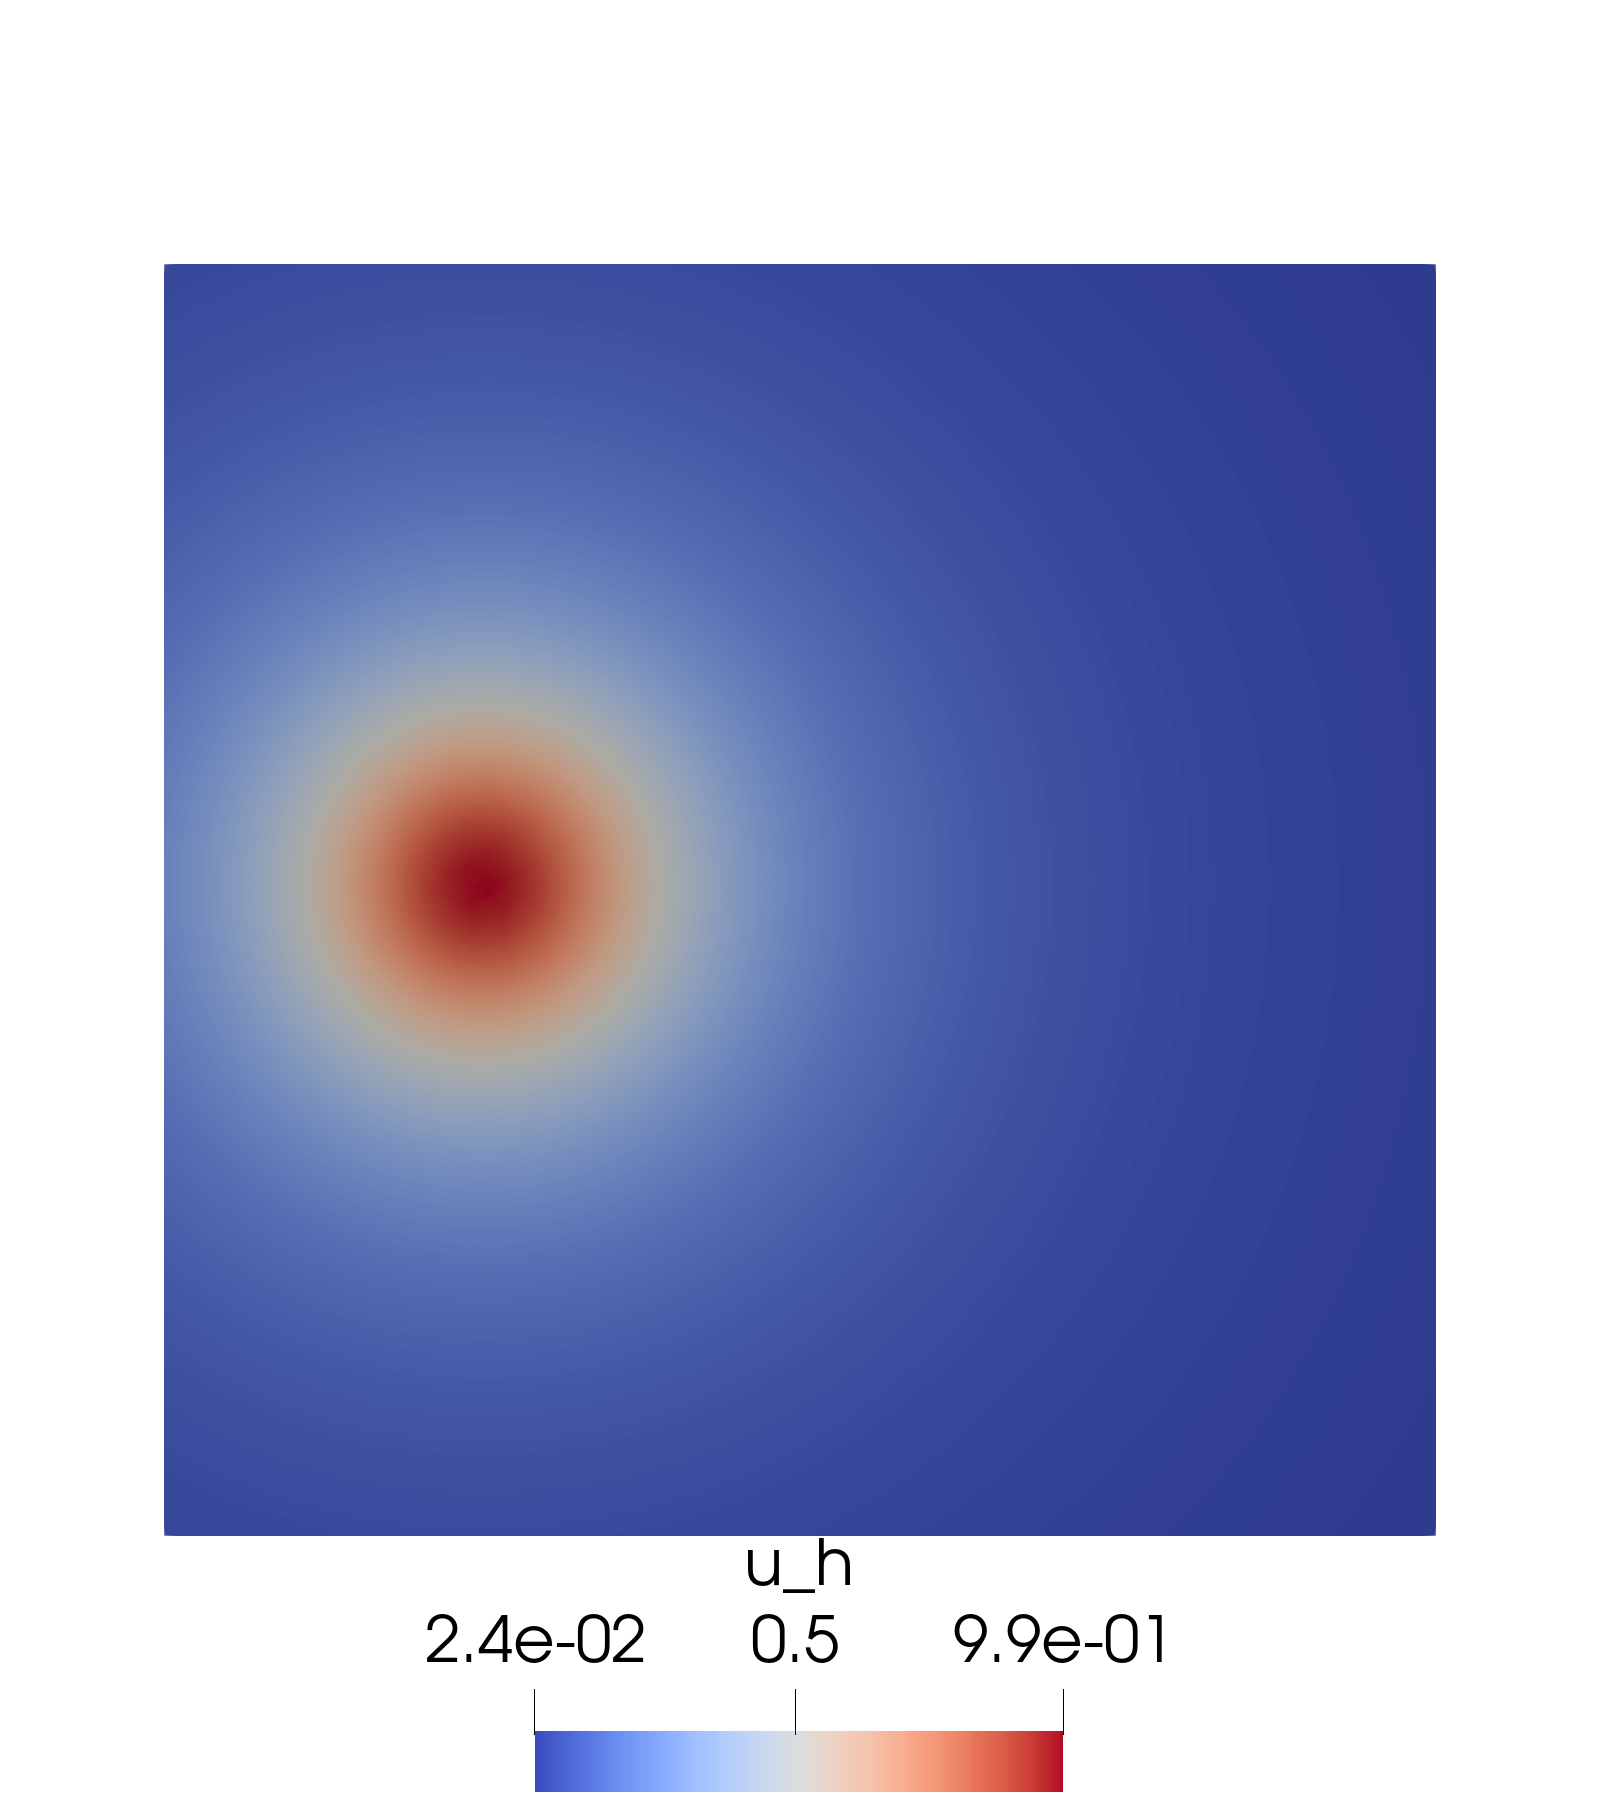
\includegraphics[width=\linewidth]{figures/heat/heat_sol.0001.png}
    \caption{$t=0.50$}
  \end{subfigure}\hfill
  \begin{subfigure}[b]{0.245\textwidth}
    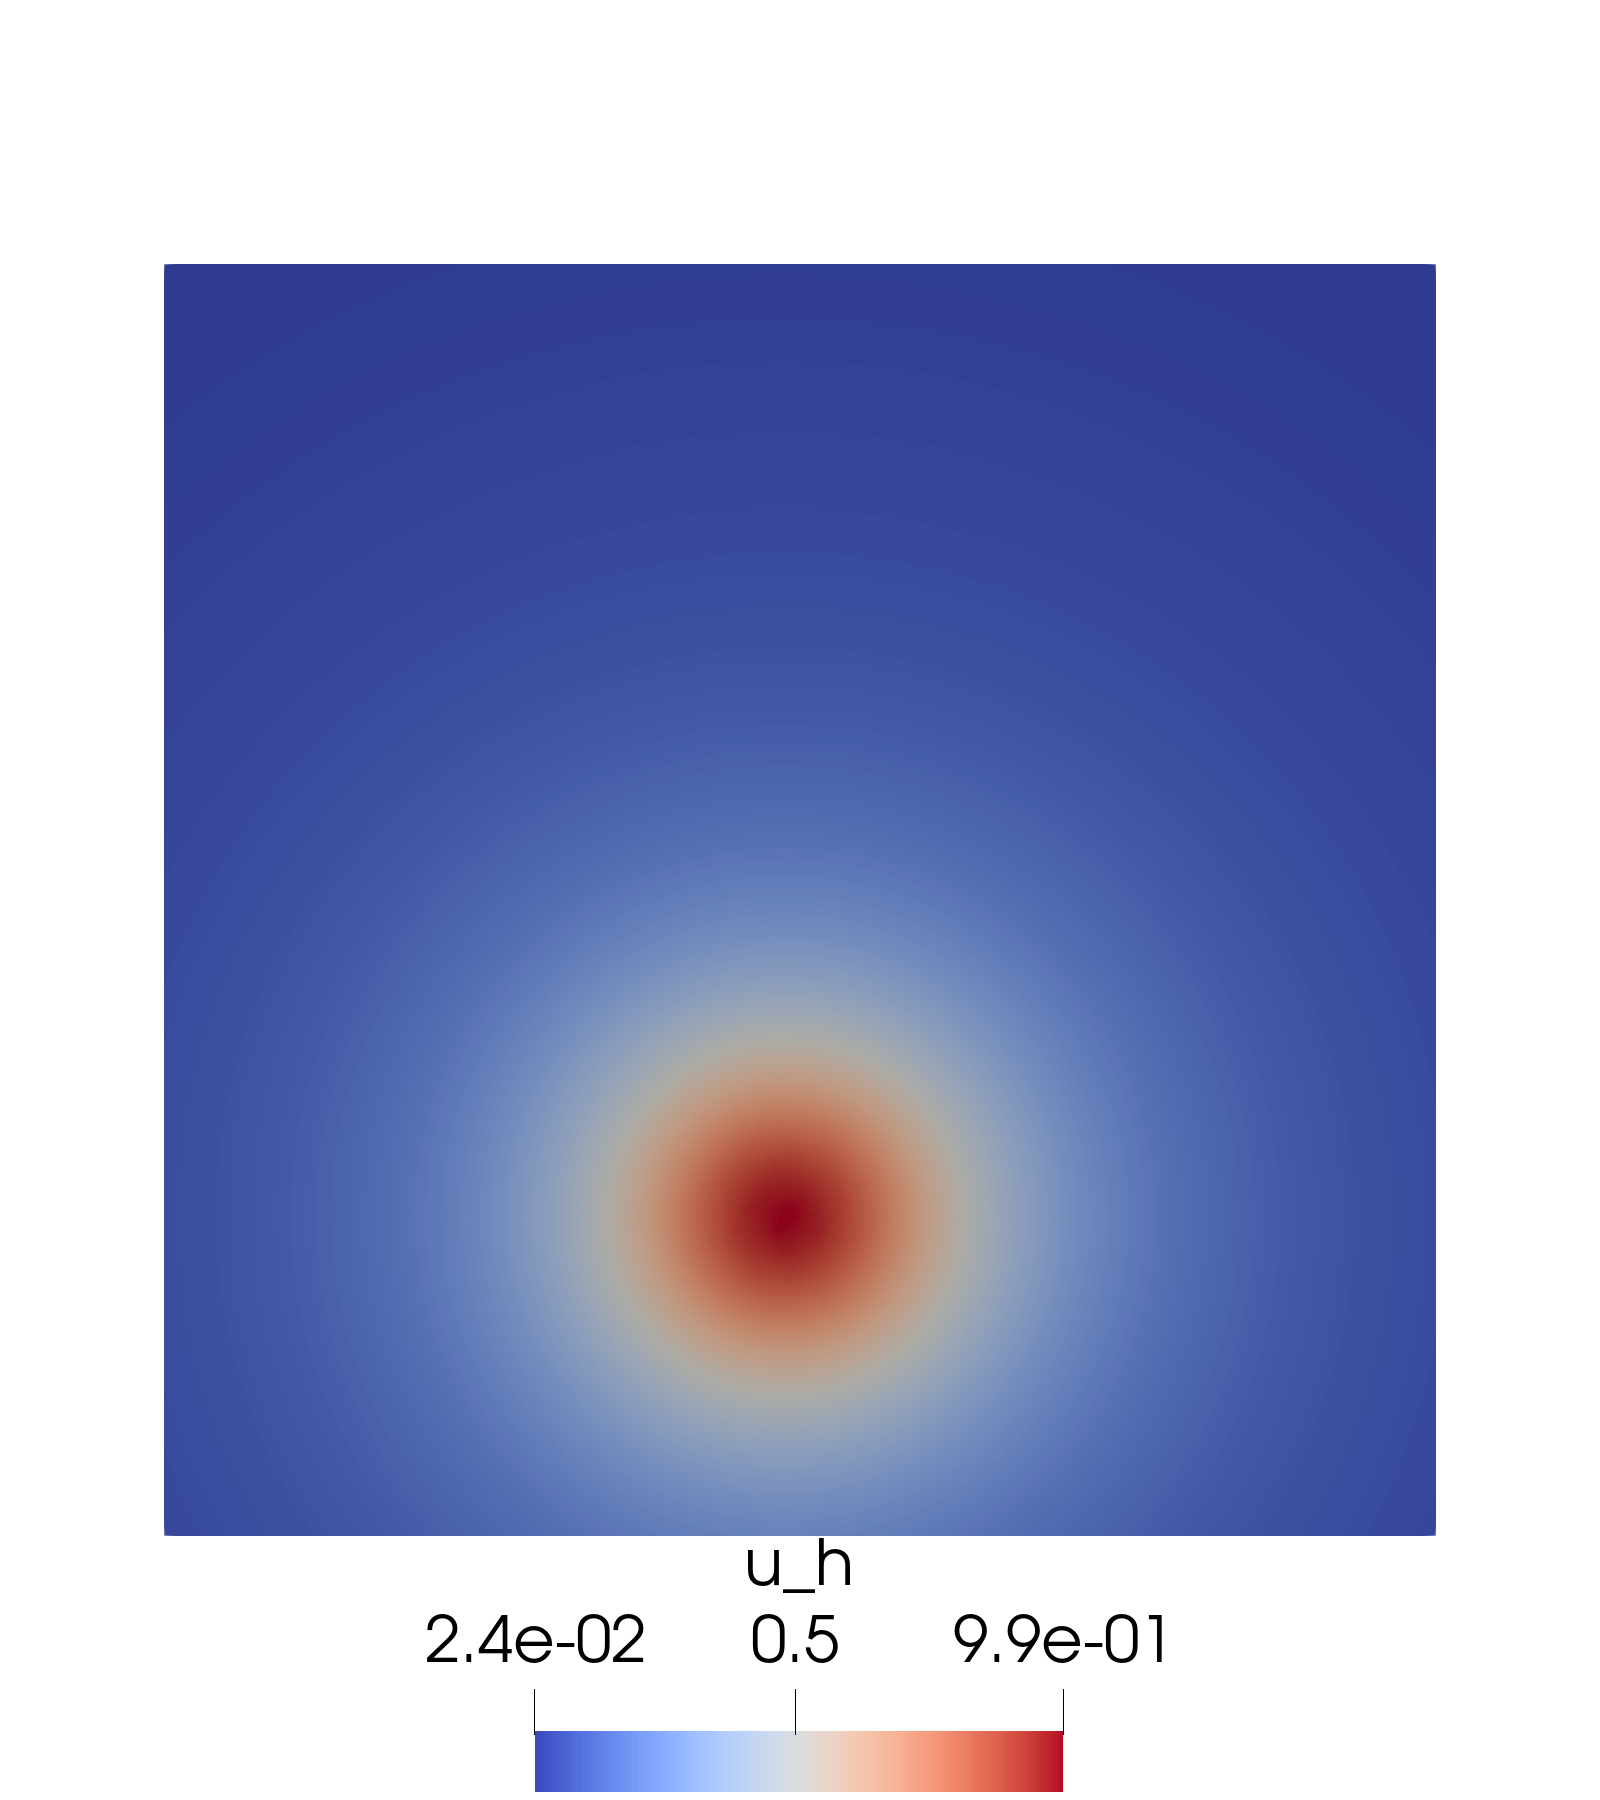
\includegraphics[width=\linewidth]{figures/heat/heat_sol.0002.png}
    \caption{$t=0.75$}
  \end{subfigure}\hfill
  \begin{subfigure}[b]{0.245\textwidth}
    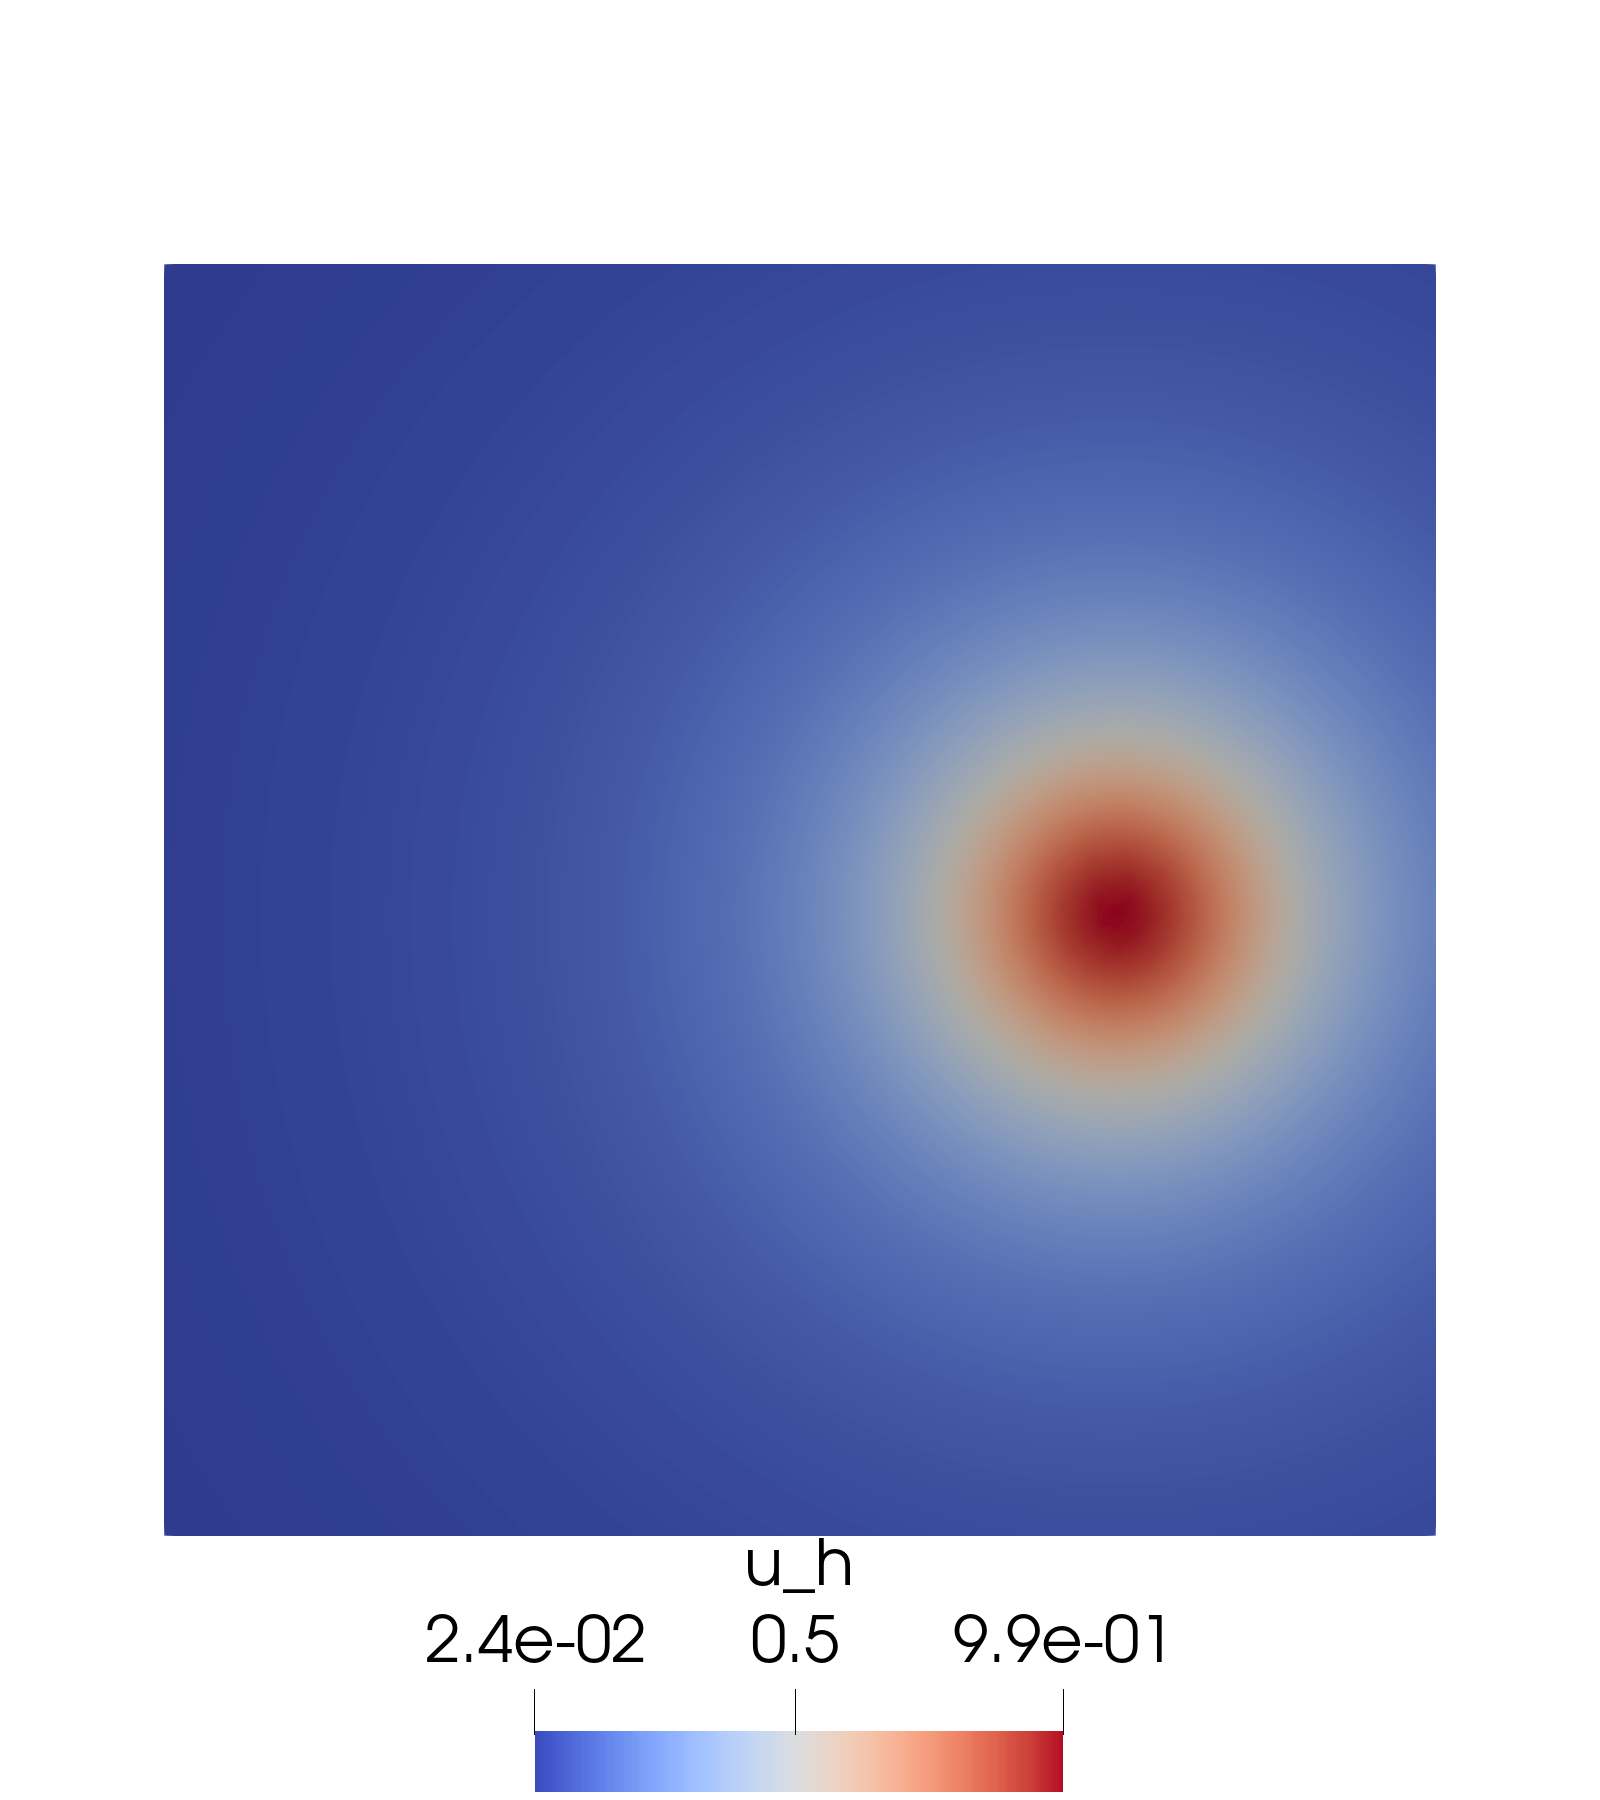
\includegraphics[width=\linewidth]{figures/heat/heat_sol.0003.png}
    \caption{$t=1.00$}
  \end{subfigure}
  \caption{Numerical rotating-hill solution at the four physical snapshot times $t=0.25,0.50,0.75,1.00$.}
  \label{fig:moving-hill-solutions}
\end{figure}
\begin{figure}[h]
  \centering
  \begin{subfigure}[b]{0.245\textwidth}
    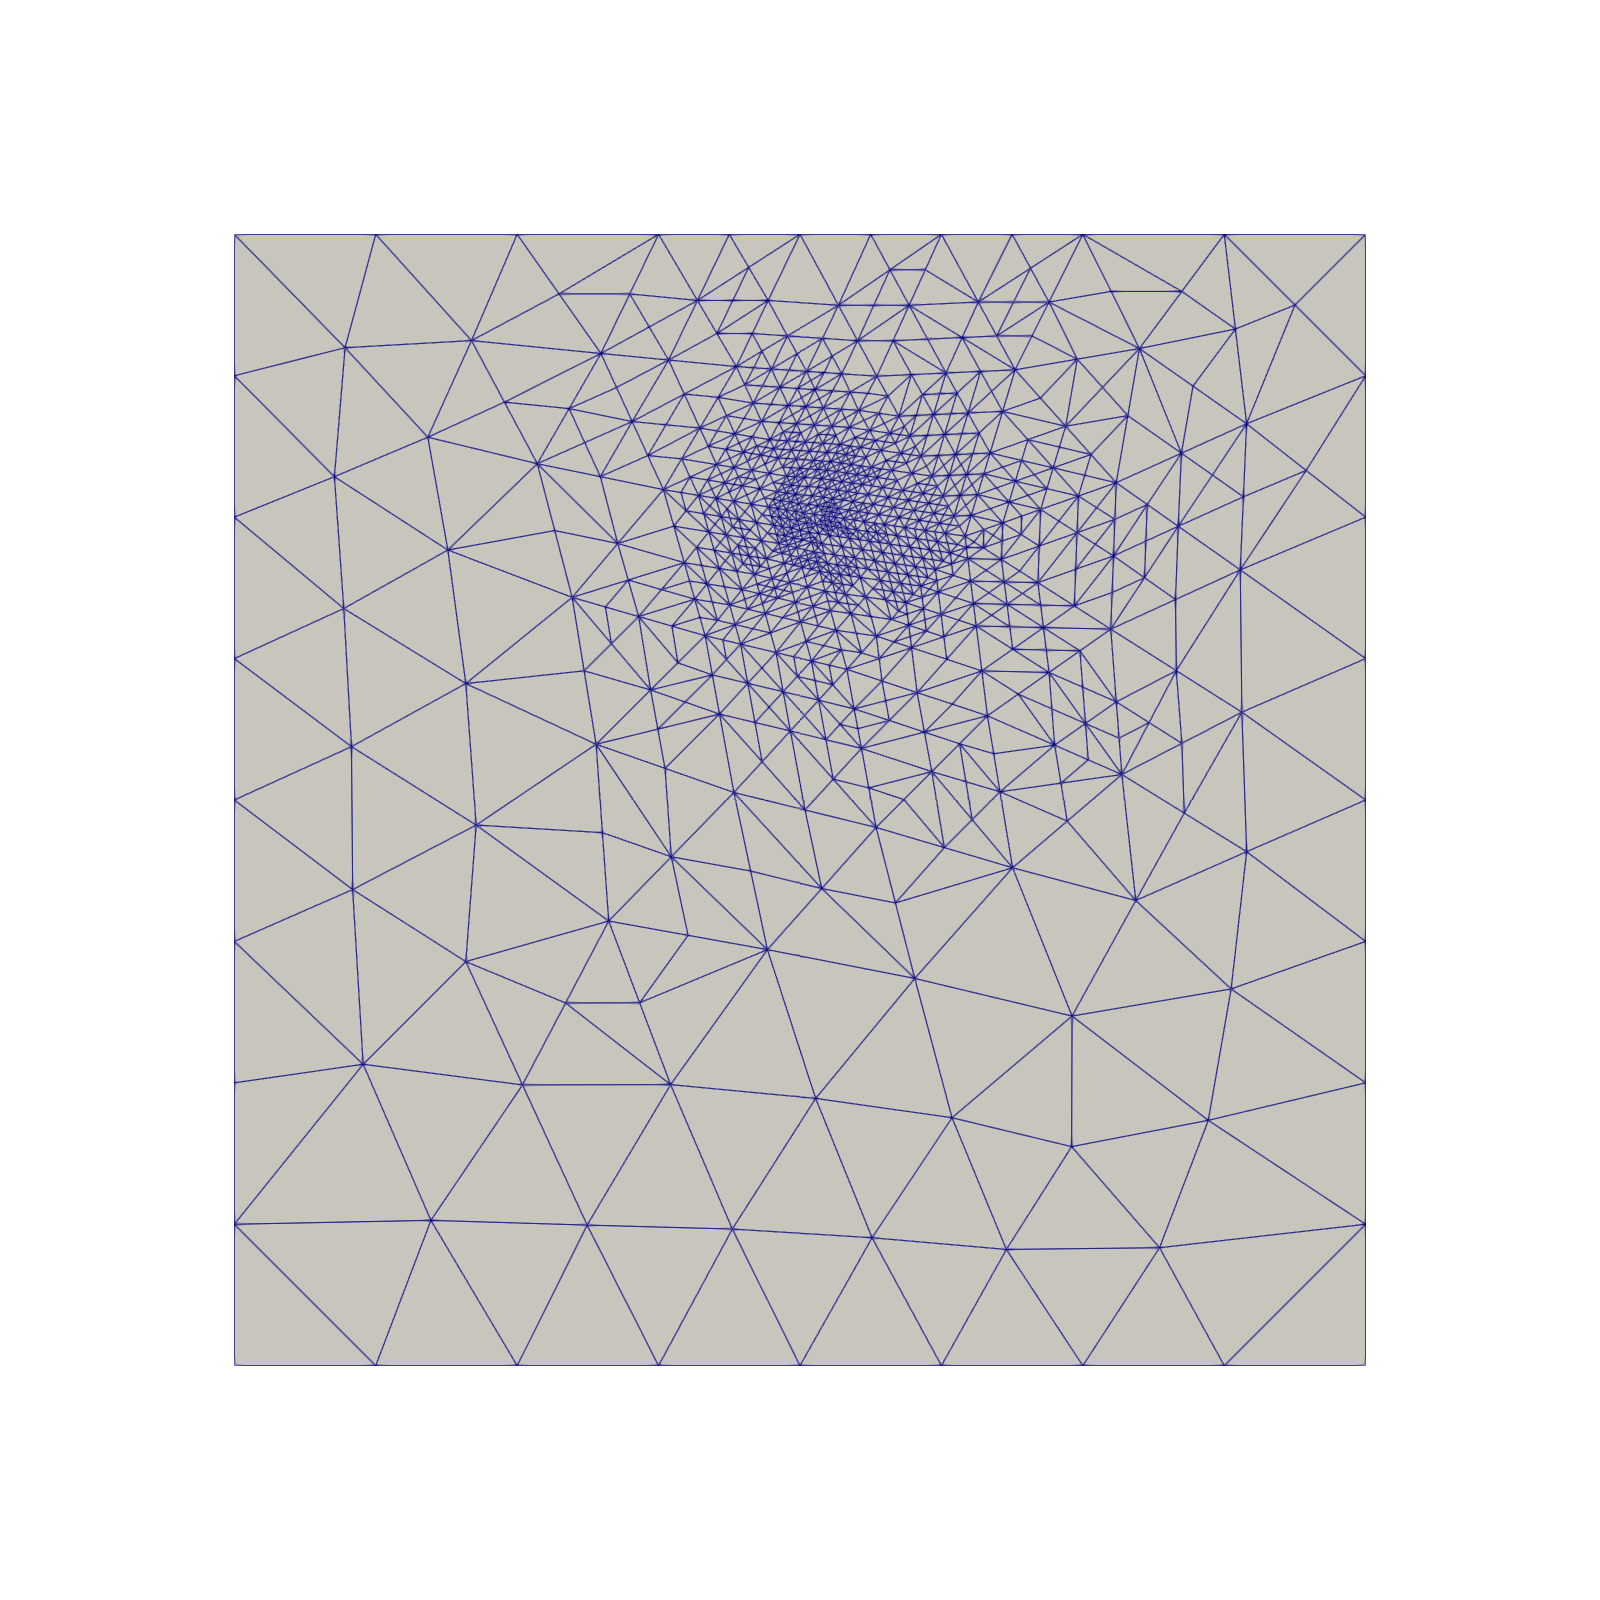
\includegraphics[width=\linewidth]{figures/heat/heat_strong.0000.png}
    \caption{$t=0.25$}
  \end{subfigure}\hfill
  \begin{subfigure}[b]{0.245\textwidth}
    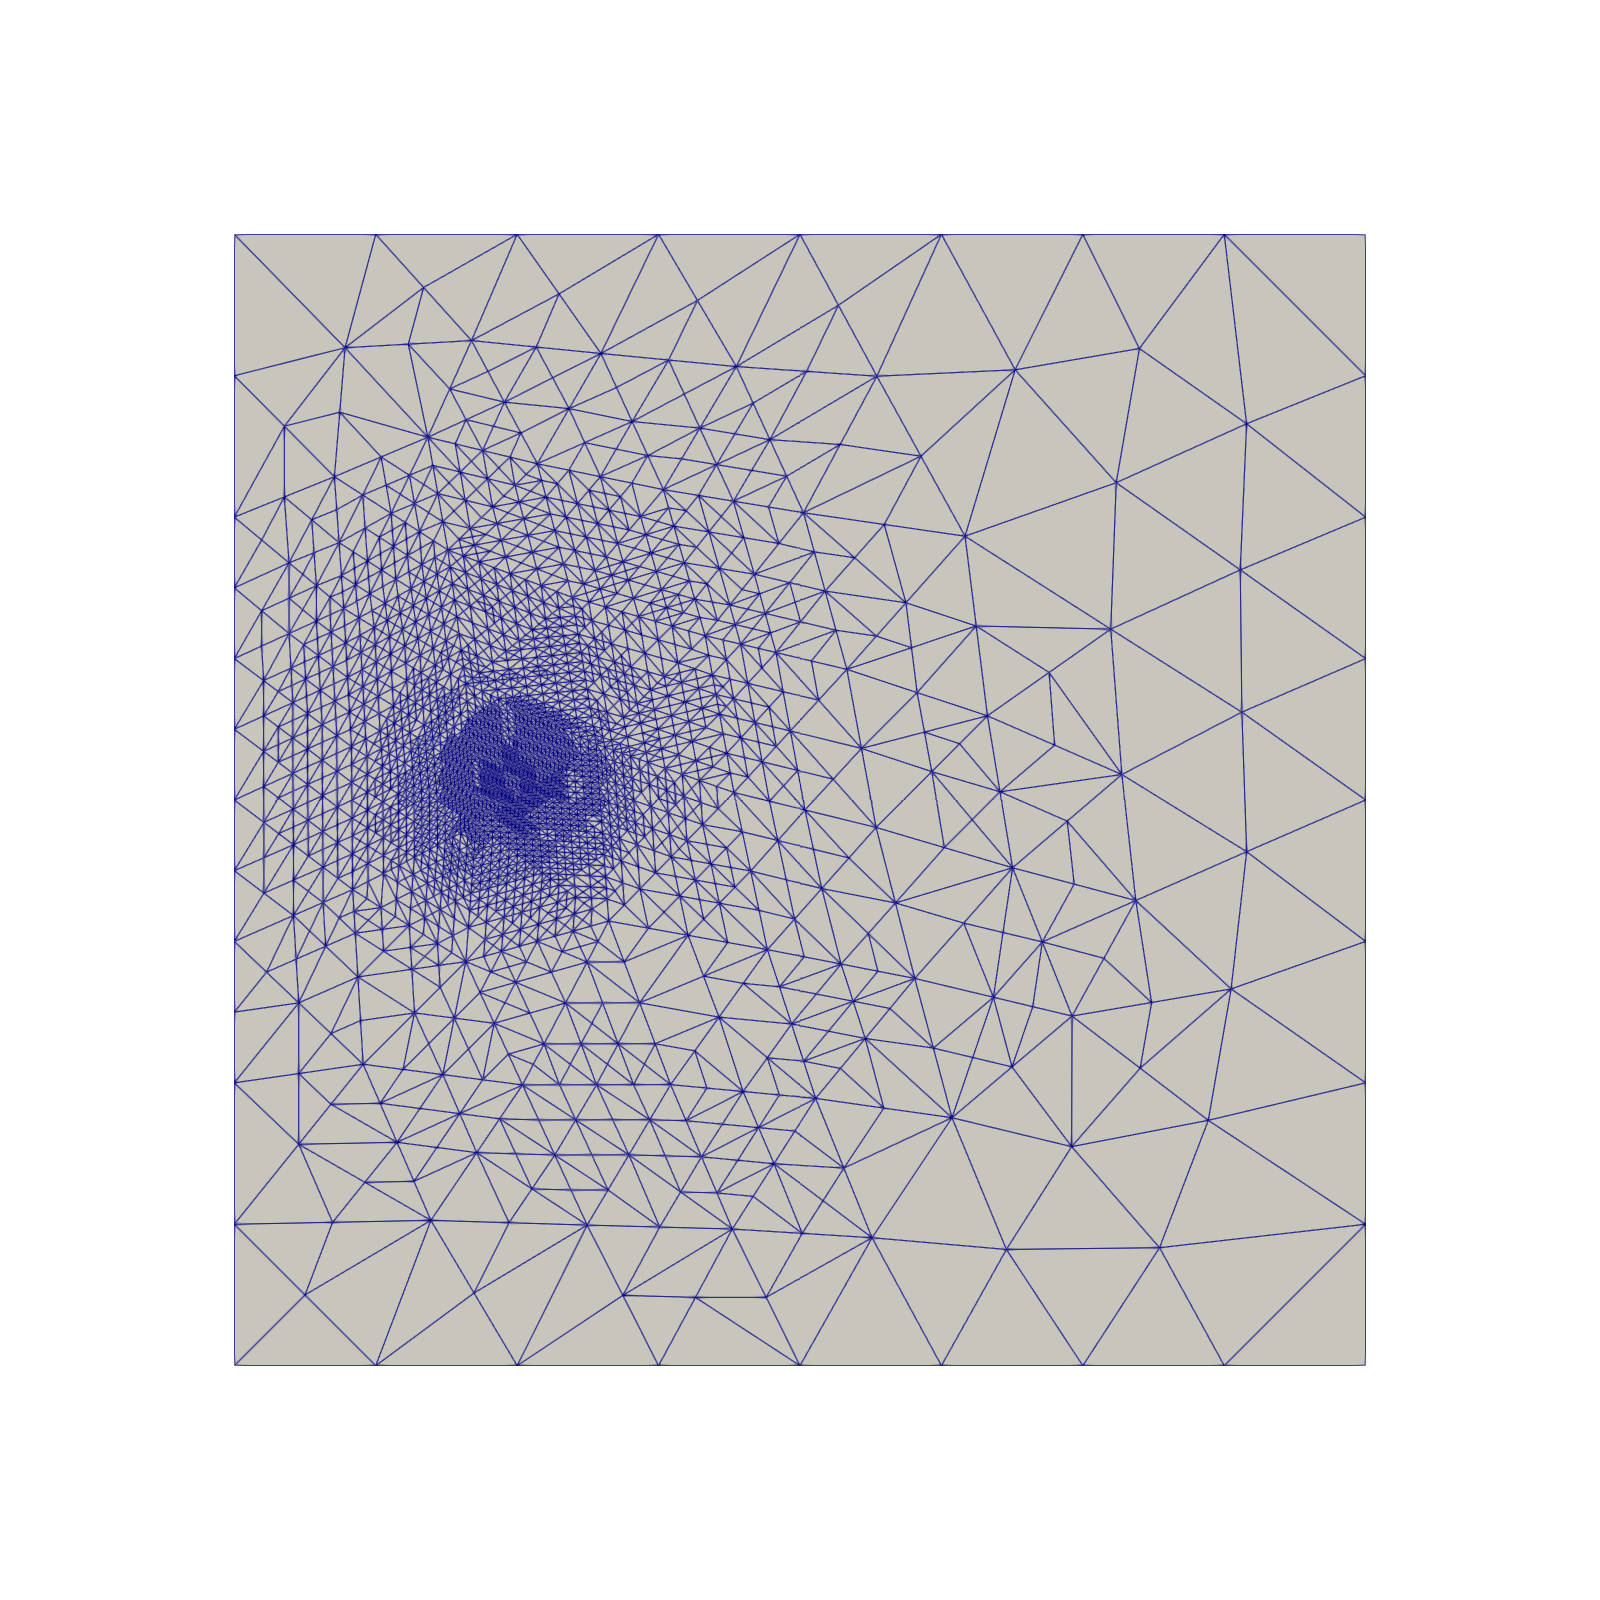
\includegraphics[width=\linewidth]{figures/heat/heat_strong.0001.png}
    \caption{$t=0.50$}
  \end{subfigure}\hfill
  \begin{subfigure}[b]{0.245\textwidth}
    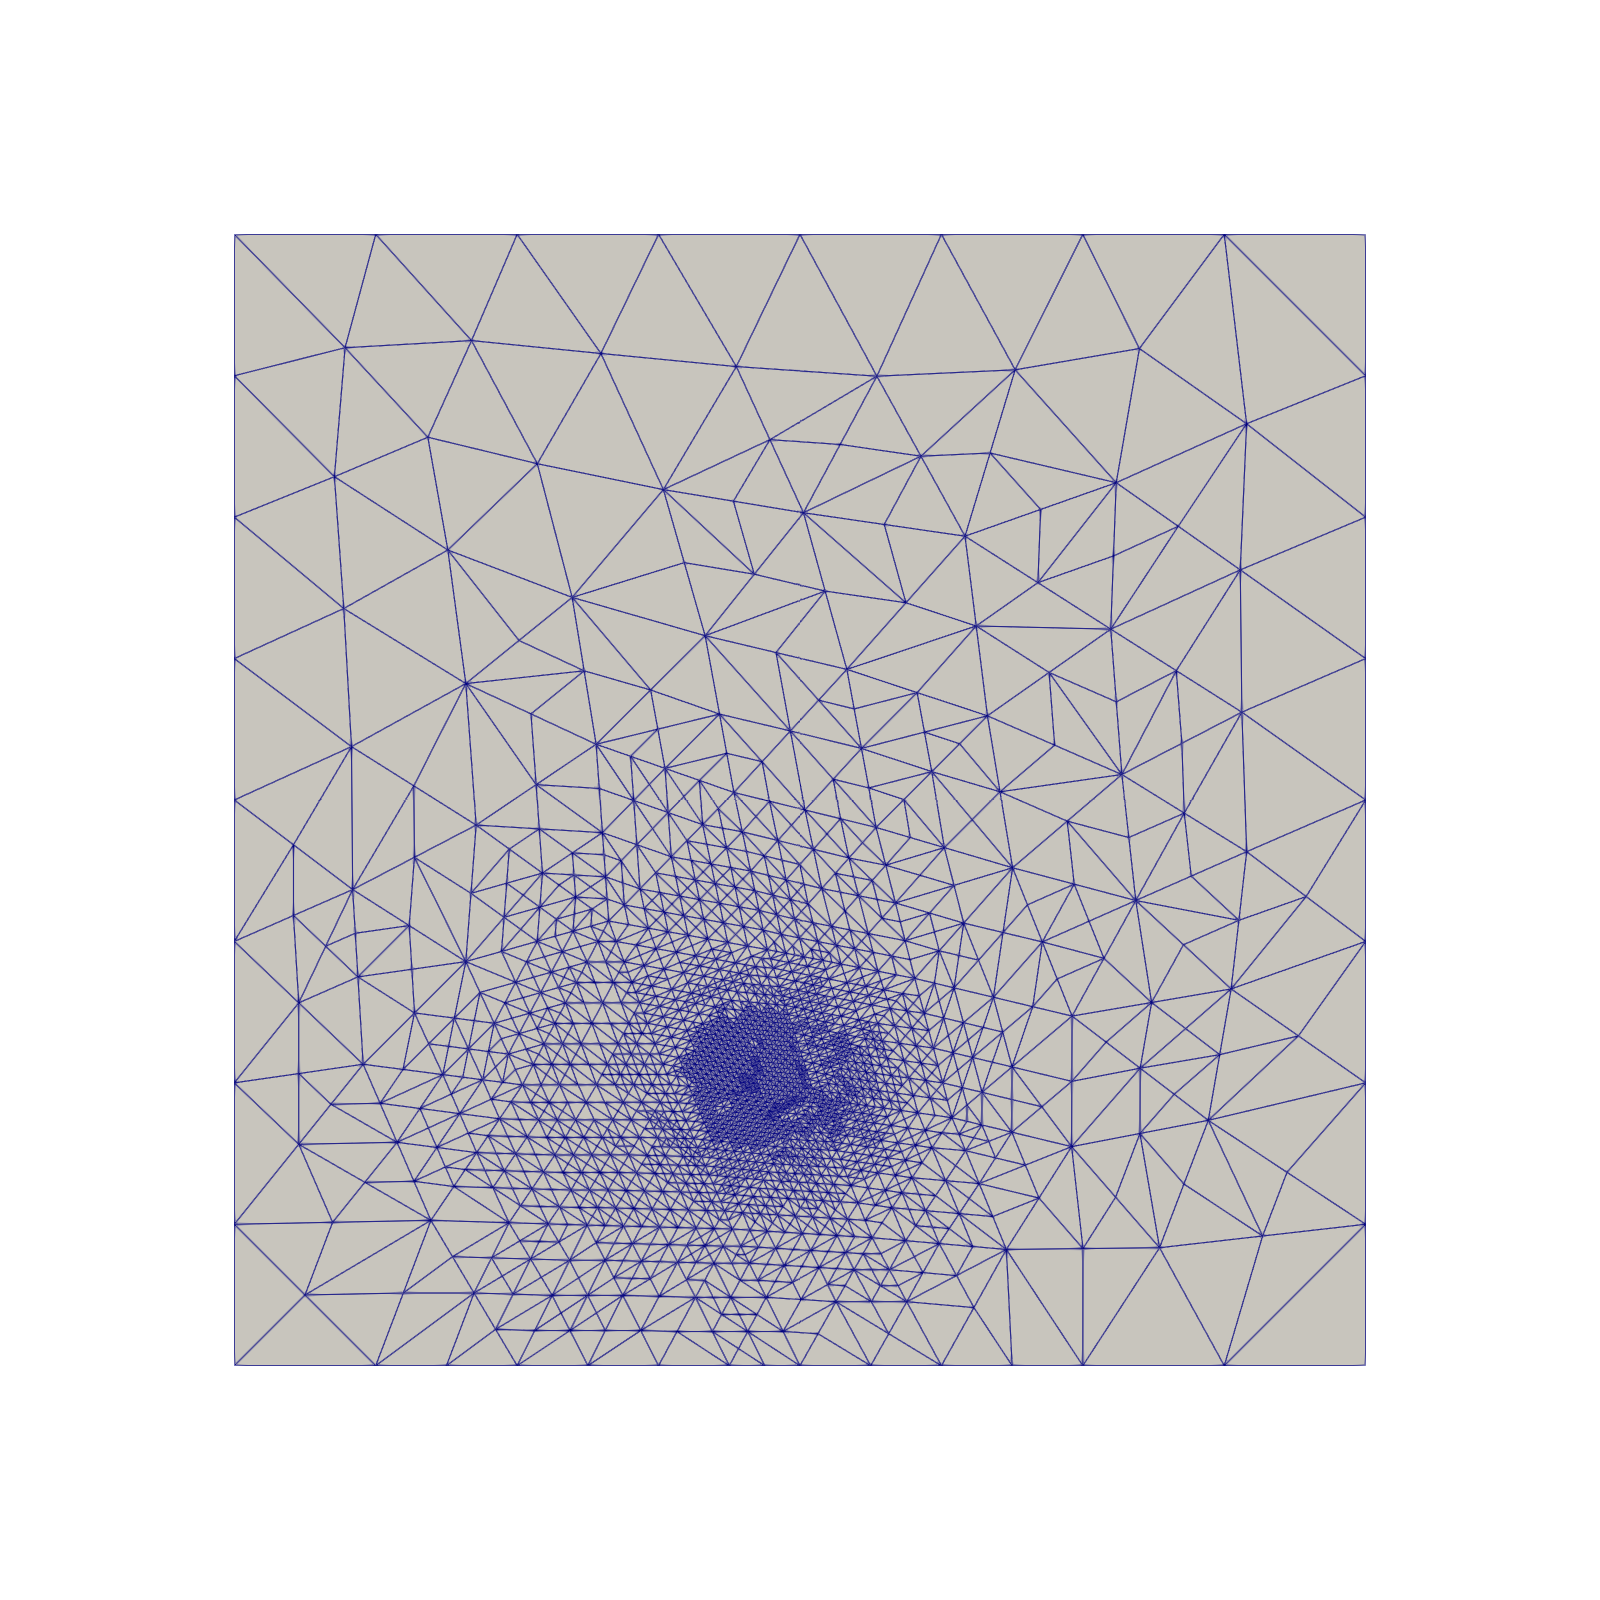
\includegraphics[width=\linewidth]{figures/heat/heat_strong.0002.png}
    \caption{$t=0.75$}
  \end{subfigure}\hfill
  \begin{subfigure}[b]{0.245\textwidth}
    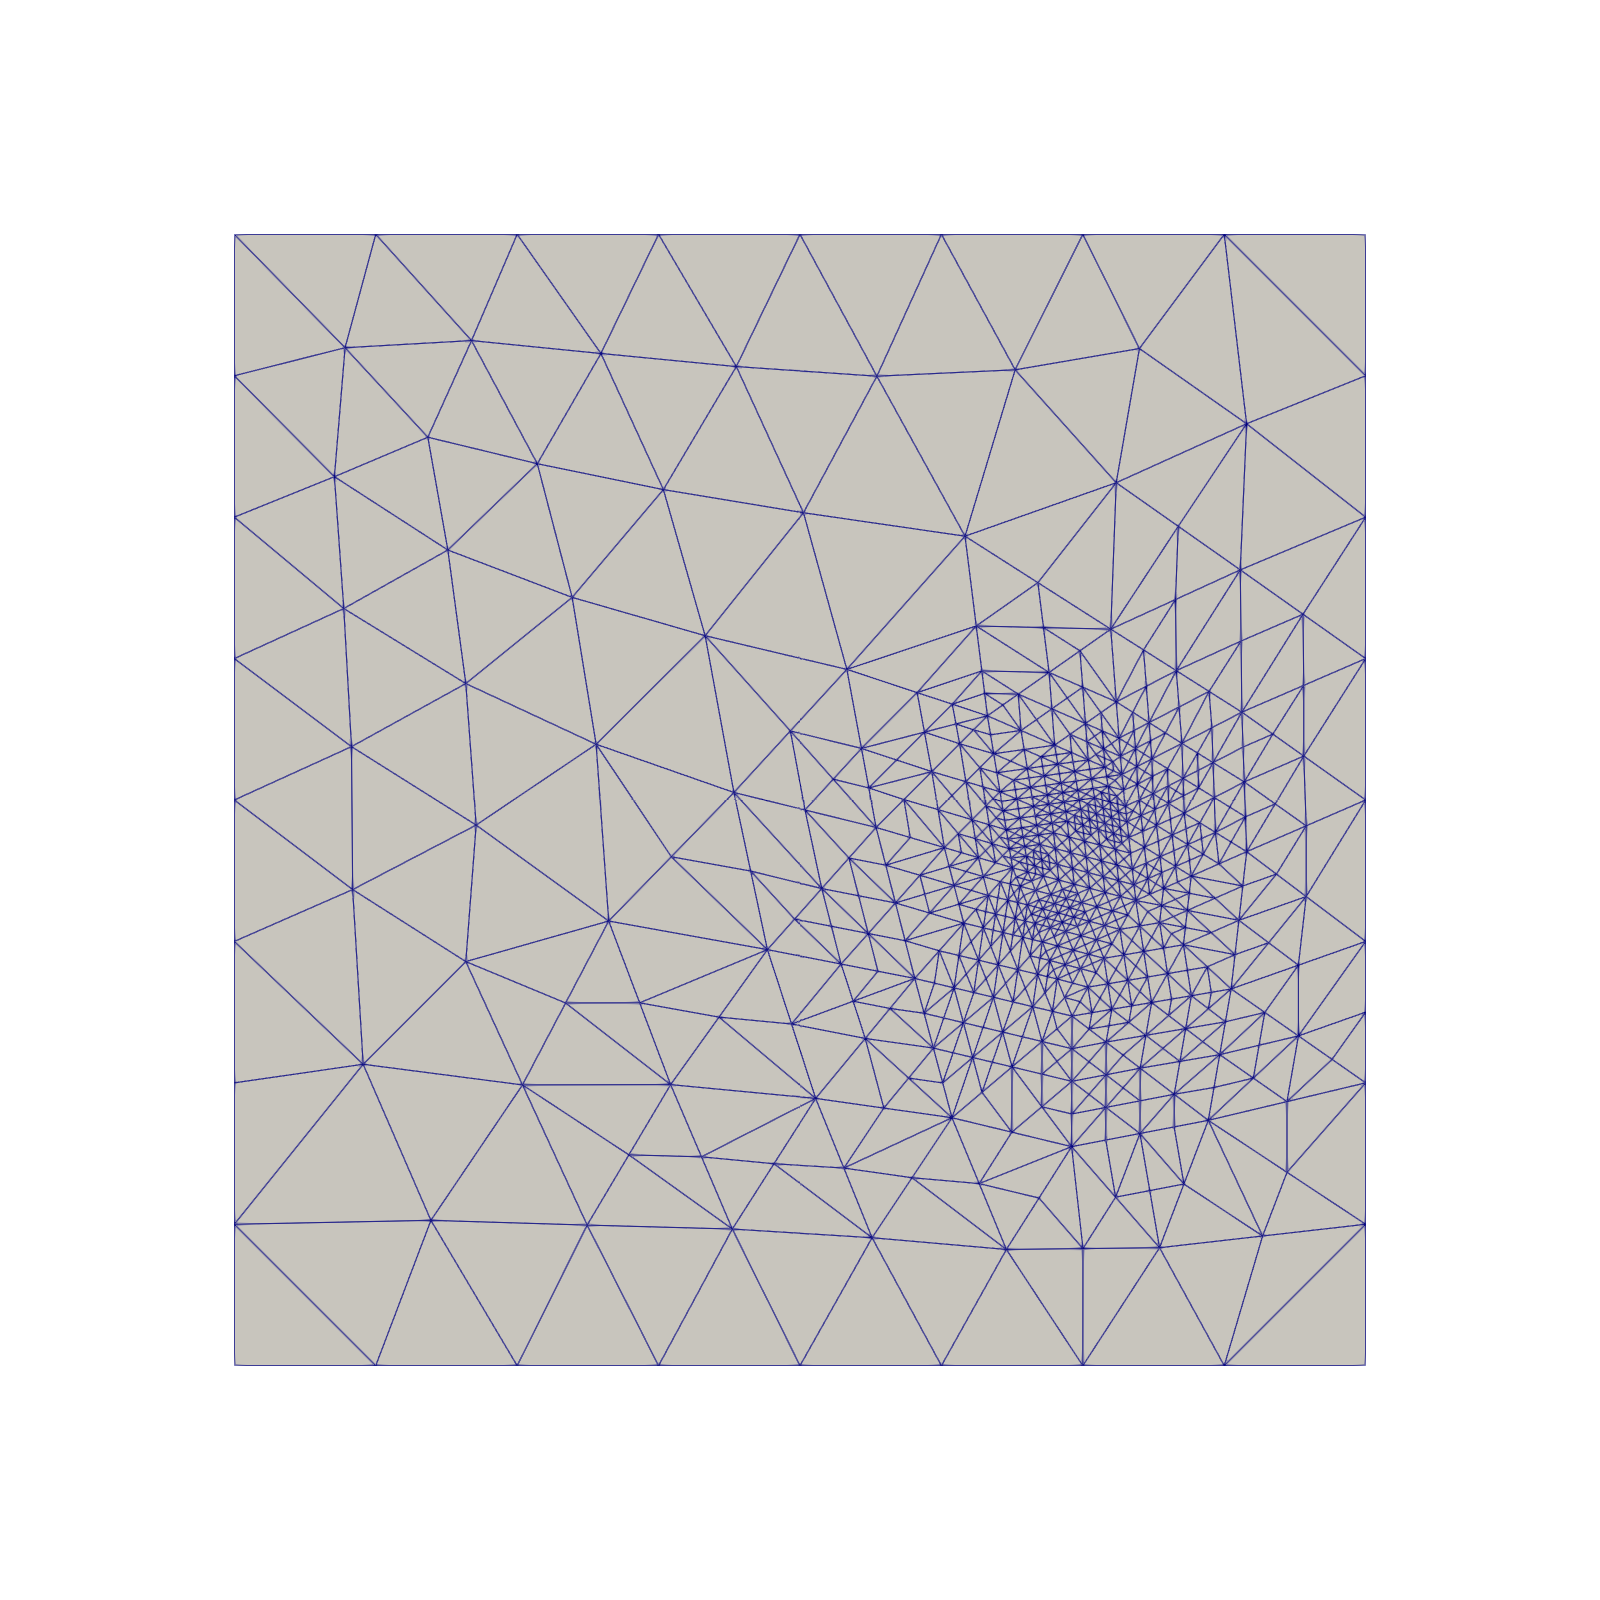
\includegraphics[width=\linewidth]{figures/heat/heat_strong.0003.png}
    \caption{$t=1.00$}
  \end{subfigure}
  \caption{Slabwise spatial meshes from strong-residual-bound marking at
  $t=0.25,0.50,0.75,1.00$ at the 8th iteration.}
  \label{fig:moving-hill-strong-meshes}
\end{figure}
\begin{figure}[h]
  \centering
  % Replace the stems below only if your exported names differ.
  \begin{subfigure}[b]{0.245\textwidth}
    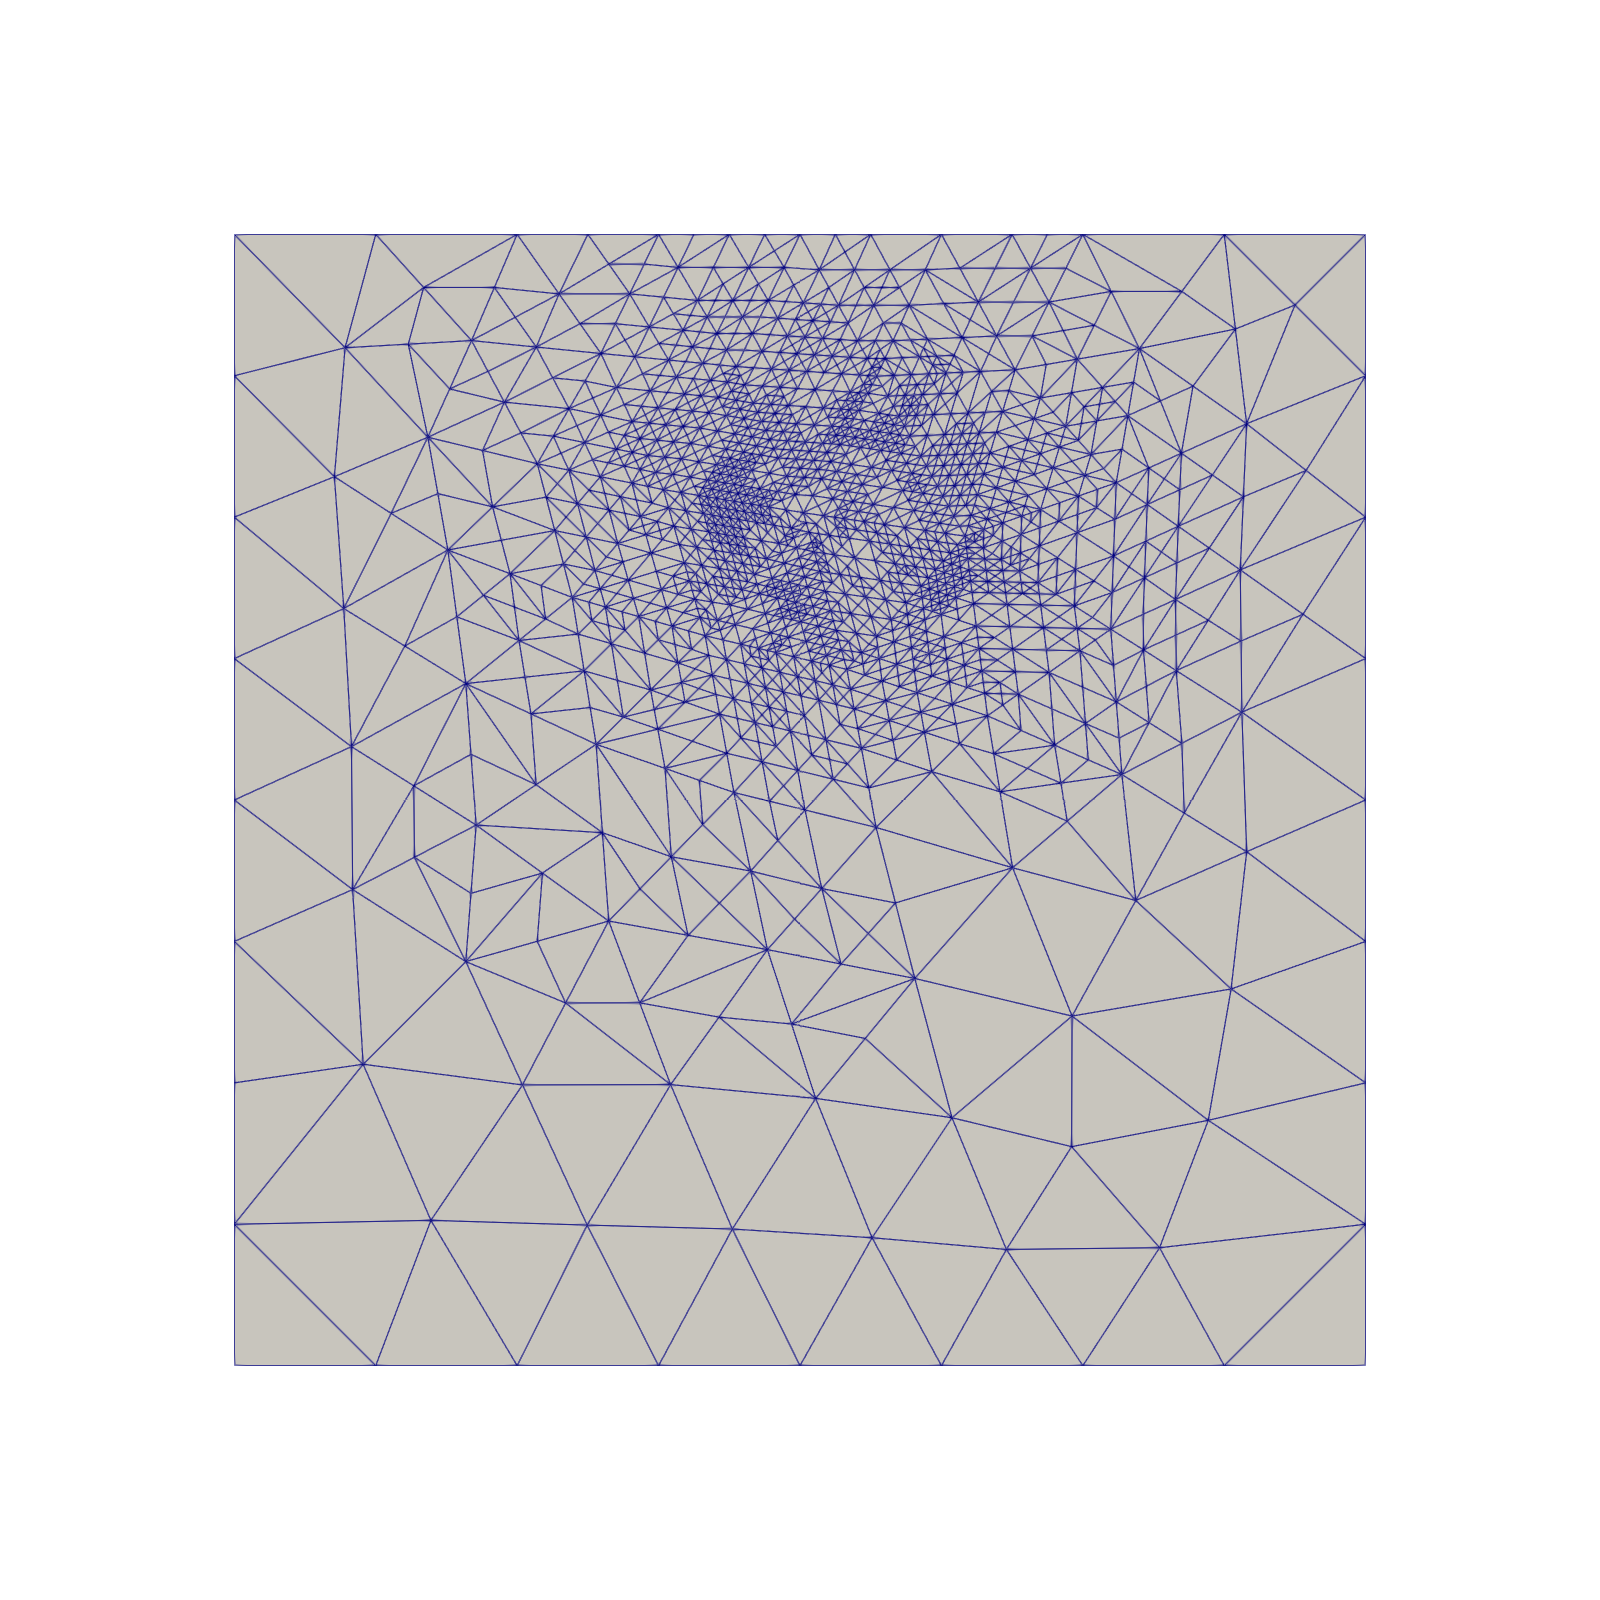
\includegraphics[width=\linewidth]{figures/heat/heat_bubble.0000.png}
    \caption{$t=0.25$}
  \end{subfigure}\hfill
  \begin{subfigure}[b]{0.245\textwidth}
    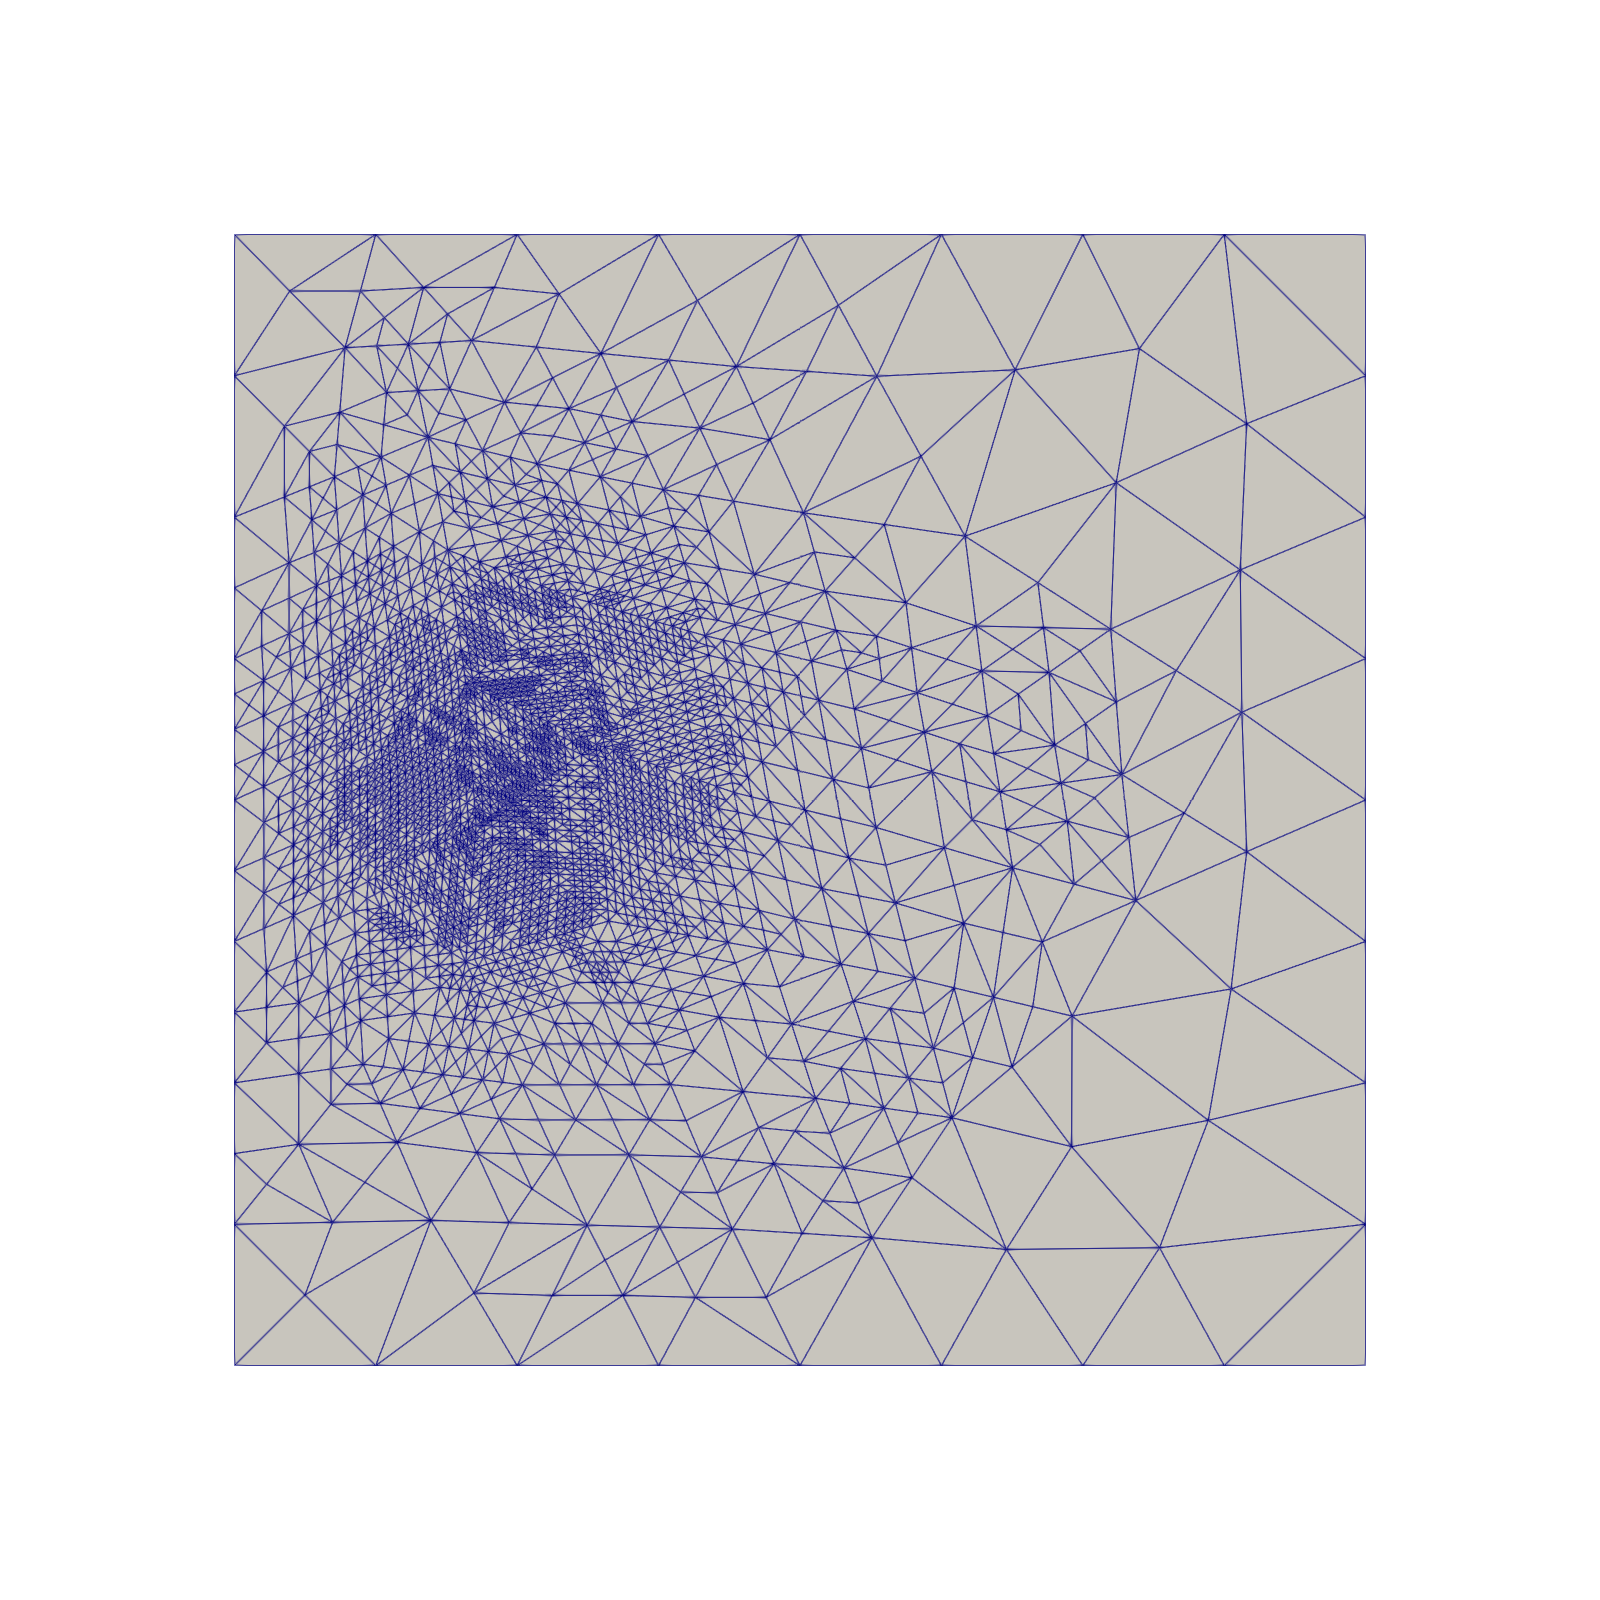
\includegraphics[width=\linewidth]{figures/heat/heat_bubble.0001.png}
    \caption{$t=0.50$}
  \end{subfigure}\hfill
  \begin{subfigure}[b]{0.245\textwidth}
    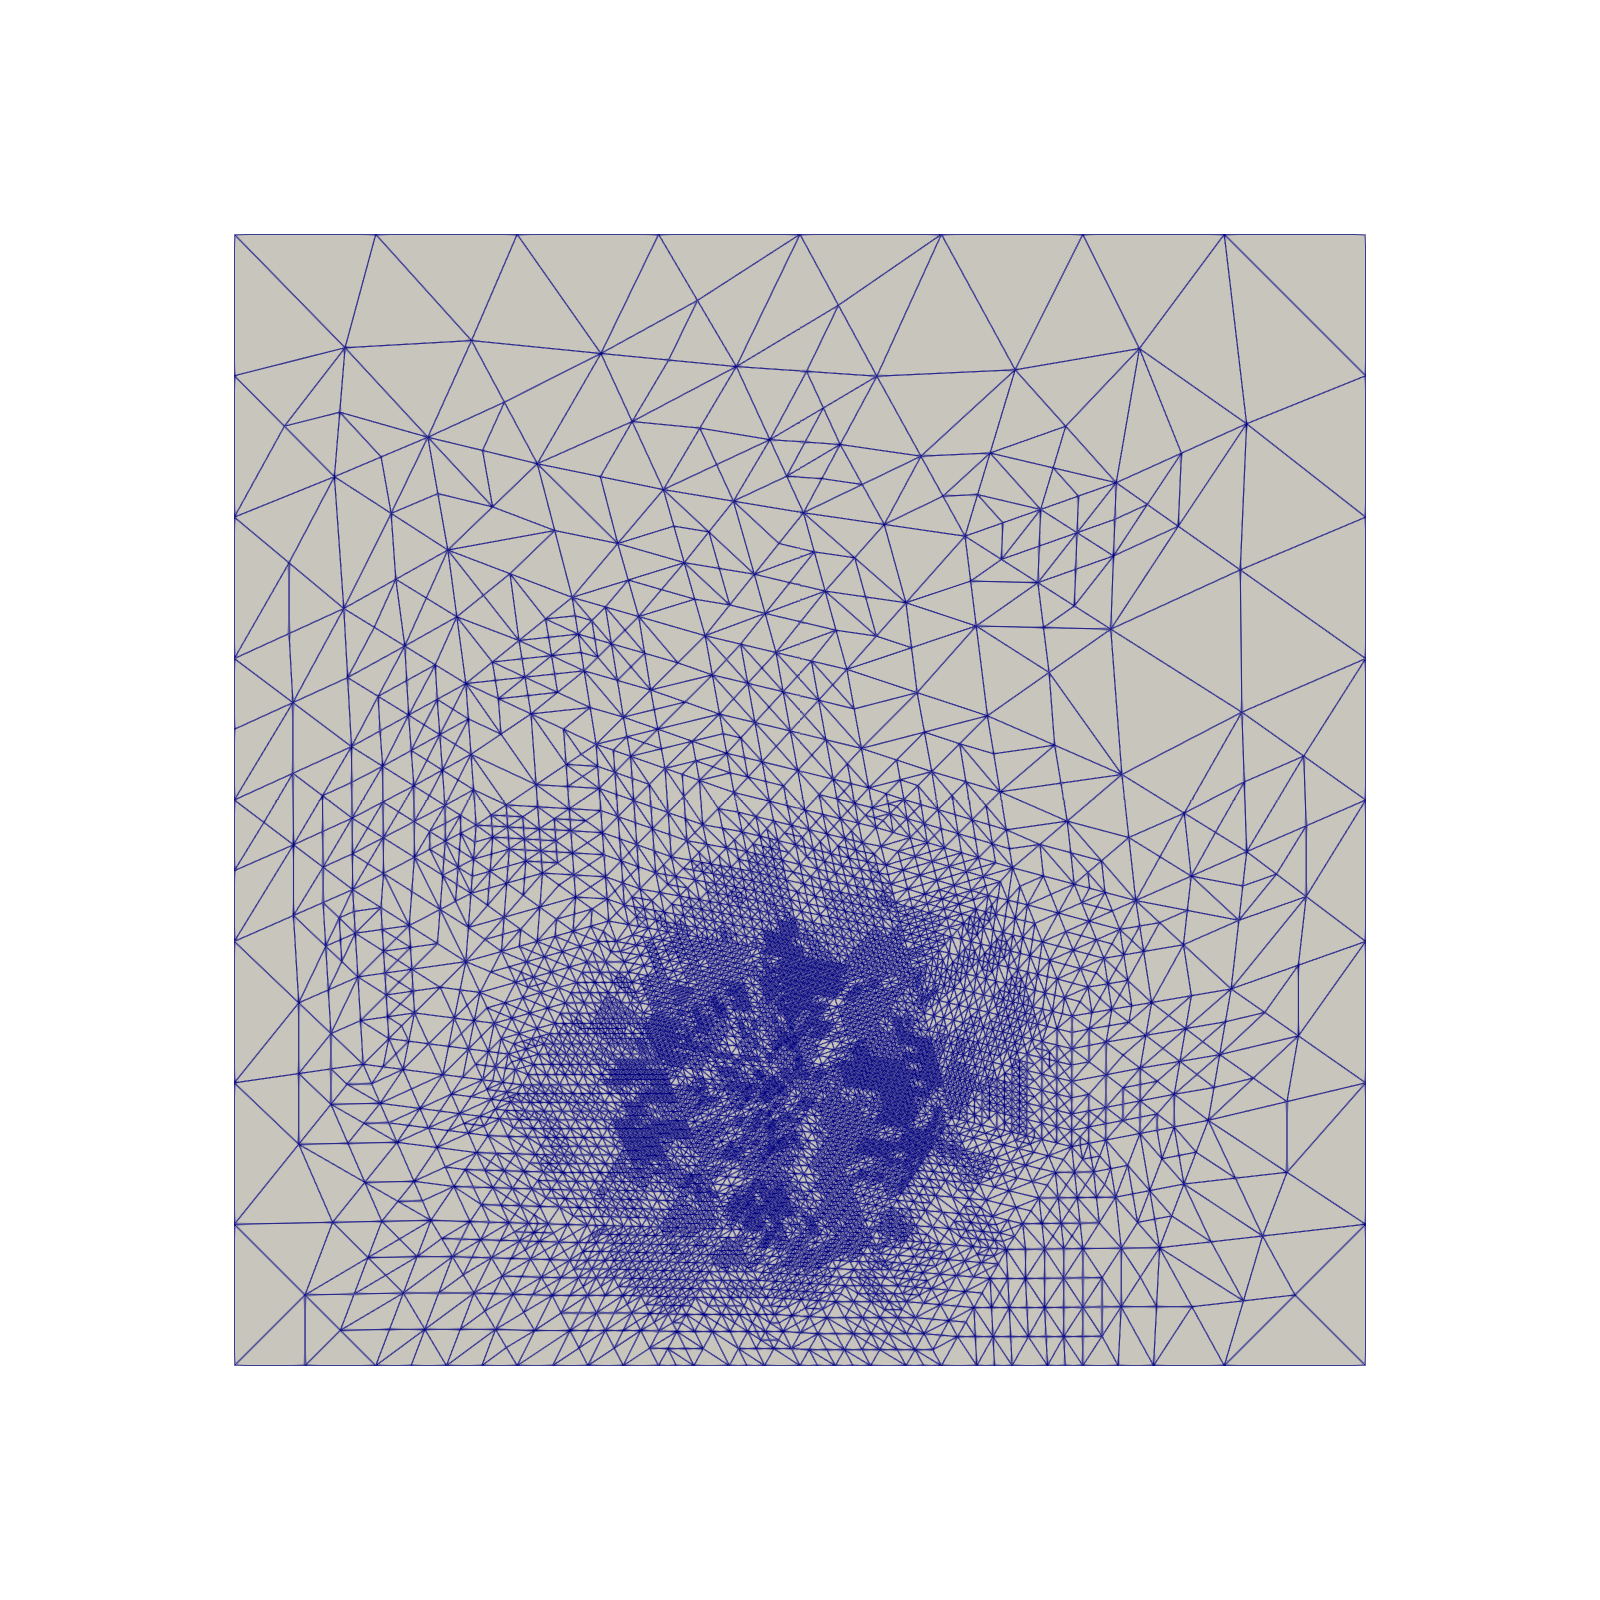
\includegraphics[width=\linewidth]{figures/heat/heat_bubble.0002.png}
    \caption{$t=0.75$}
  \end{subfigure}\hfill
  \begin{subfigure}[b]{0.245\textwidth}
    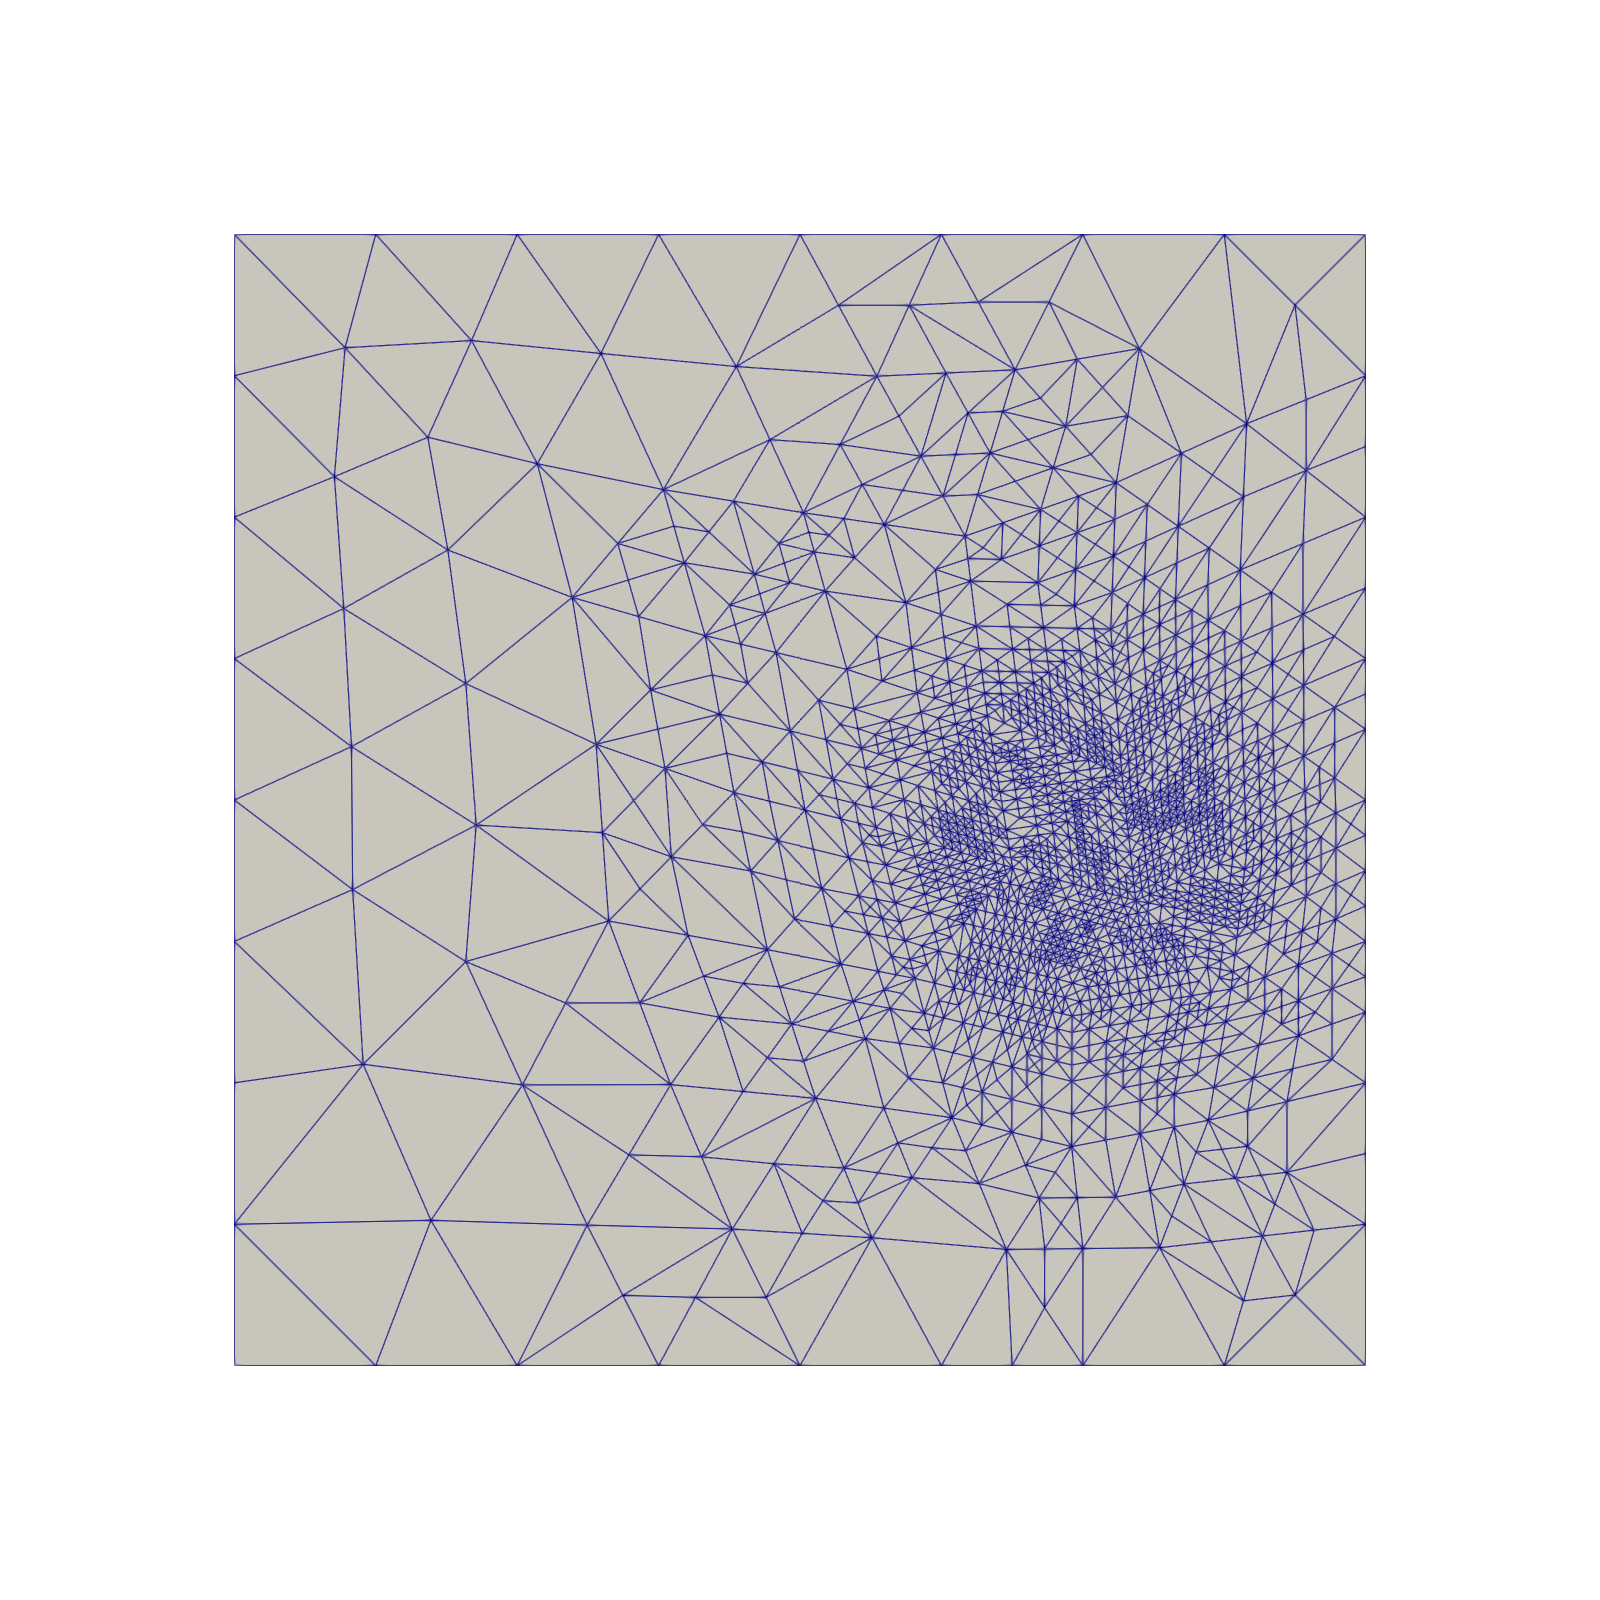
\includegraphics[width=\linewidth]{figures/heat/heat_bubble.0003.png}
    \caption{$t=1.00$}
  \end{subfigure}
  \caption{Slabwise spatial meshes from the bubble run at the physical snapshot times $t=0.25,0.50,0.75,1.00$ at the 8th iteration.}
  \label{fig:moving-hill-bubble-meshes}
\end{figure}

For both localisation methods, the refined spatial regions follow the moving hill. The strong-residual indicator is a positive upper-bound quantity constructed from residual and dual-weight norms. Under the present marking rule, all space--time cell indicators are sorted in descending order and the largest entries are selected until their cumulative sum reaches $\theta=0.4$ of the total indicator activity. The strong-residual activity is concentrated in fewer large entries and therefore produces fewer, more compact spatially refined regions.
The bubble localisation combines signed recovered volume, spatial-trace and temporal-trace contributions. These components may partially cancel in the final cell indicator. Moreover, recovered facet contributions are assigned to neighbouring cells, which can distribute the indicator activity over a wider spatial region. This could explain why more cells are selected and why the bubble meshes display broader refined patches around the moving-hill trajectory in this experiment.

The results motivate a componentwise marking indicator,
\[
m_{K,n}^{\rm comp}
 =
 |\eta_{\rm vol}|
 +|\eta_{\rm spatial}|
 +|\eta_{\rm temporal}|
 +|\eta_{\rm mixed}|.
\]
This modification prevents large entity contributions from being hidden by local sign cancellation and may therefore provide a more robust refinement indicator in cases where the recovered components have competing signs. However, it may also mark unexpected regions and increase computational cost, so its benefit must be assessed experimentally rather than assumed.
